%!TEX root = /Users/stevenmartell/Documents/iSCAM-project/fba/Halibut/WRITEUP/Halibut.tex

\section{Results} % (fold)
\label{sec:results}

The initial numbers-at-age, age-1 recruits, fishing mortality rates and size selectivity parameters were all used to initialize this simulation model.  Estimates of the sex/age-specific total mortality rates between this simulation model and the wobblesq model are nearly identical.  Trends in exploitable biomass between the two models differ due to at least two factors (Figure \ref{fig:FIGURES_EBioDemo}): age-smearing and differences in the weight-at-age data used to calculate exploitable biomass.  In the IPHC assessment model, the annual calculation of exploitable biomass is based on the predicted numbers-at-age with aging error (smearing) times the empirical weight-at-age data from the commercial fishery.  The simulation model does not use an age-misclassification matrix to smear the numbers at age, and the weight-at-age data is based on the allometric length-weight relationship and the empirical mean length-at-age data from the setline survey.  The net results is that the predicted exploitable biomass in the simulation model is less than the predicted exploitable biomass from the IPHC assessment (Figure \ref{fig:FIGURES_EBioDemo}).

\begin{figure}[htbp]
	\centering
		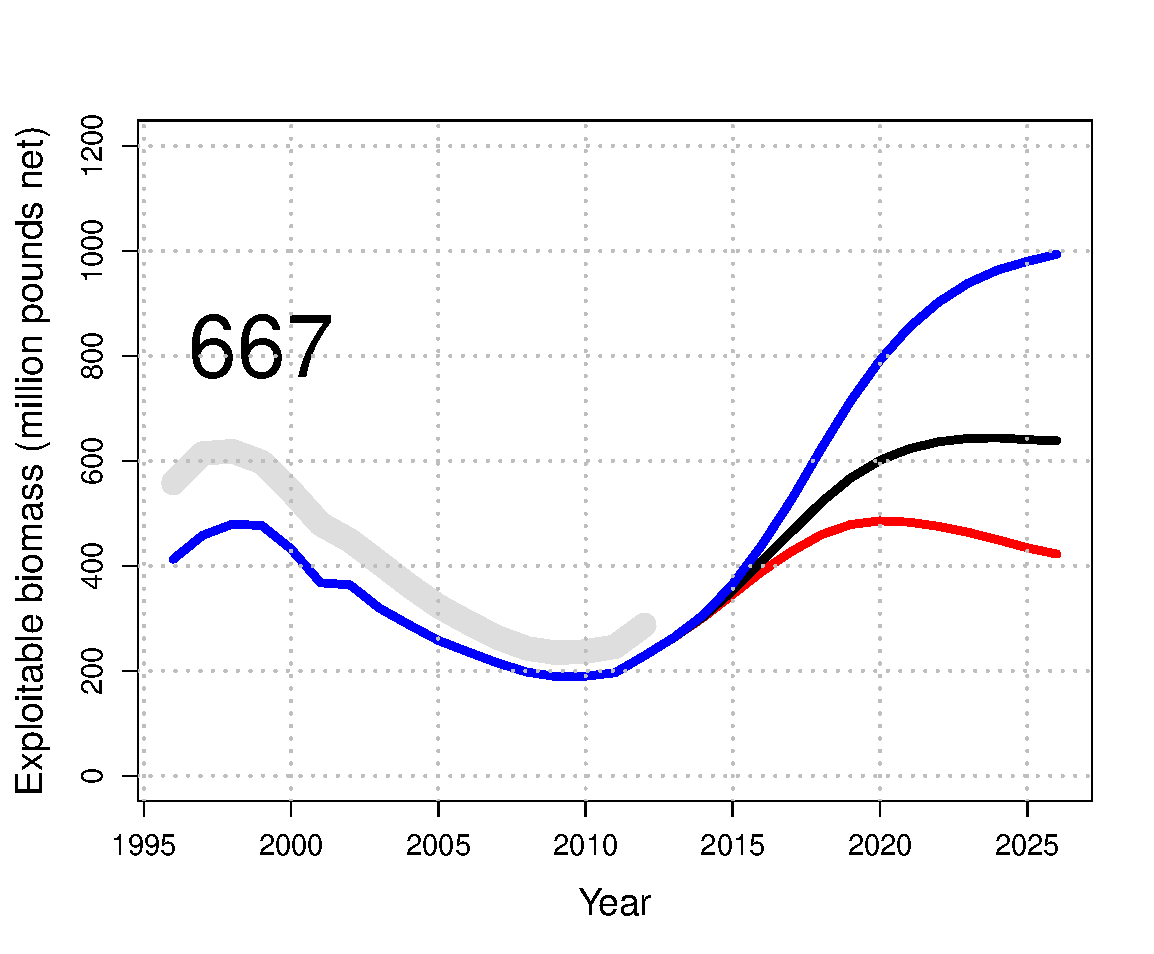
\includegraphics[height=3in]{../FIGURES/EBioDemo.pdf}
	\caption{Example of simulation model output for the exploitable biomass under poor, average and good recruitment. The thick grey line is the exploitable biomass output from the IPHC wobblesq assessment conducted at the end of the 2011 fishing season. }
	\label{fig:FIGURES_EBioDemo}
\end{figure}

Figure \ref{fig:FIGURES_EBioDemo} summarizes the results of the status quo scenario for the exploitable biomass, where 667 million pounds is the average predicted biomass over all three recruitment hypotheses with density independent growth. This figure is the prototype that will be used to examine all response variables to simulated bycatch reductions.

The effect of increase recruitment density of each simulated cohort on growth rates is summarized in Figure \ref{fig:FIGURES_fig:growth}.  The asymptotic length of each cohort is a function of relative cohort density; with high densities the asymptotic length decreases.   For example the an age-15 female halibut can weigh as little as 15.3lb. at high recruitment densities and as much as 42.8lb. at low recruitment density.  Density-dependent growth has a large effect on the calculation of exploitable biomass, largely due to the increase in proportion of males that are now vulnerable to the fishing gear.  Whereas, density-dependent growth is less important in the calculation of female spawning biomass, as females grow much faster and larger than males.

\begin{figure}[htbp]
	\centering
		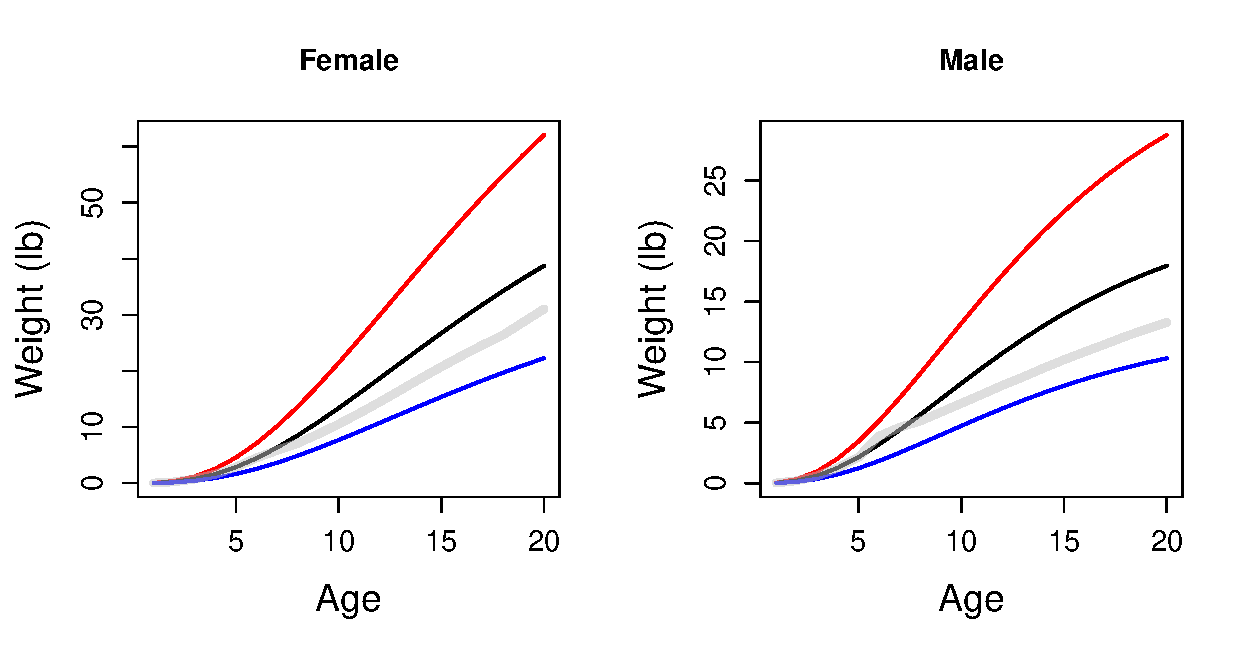
\includegraphics[height=3in]{../FIGURES/fig:growth.pdf}
	\caption{Simulated weight-at-age for halibut under low recruitment densities (red), average recruitment densities (black), and high recruitment densities (blue).}
	\label{fig:FIGURES_fig:growth}
\end{figure}



% ----------------------------------------------------------------------------- %
\subsection{Effects of bycatch reduction on EBio} % (fold)
Overall, reducing bycatch in BSAI or the GULF by 50\% has very little effect on the coastwide exploitable biomass.  The average exploitable biomass between 2020 and 2025 ranged from 597 million lbs to 667 million lbs (Figure \ref{fig:FIGURES_fig_SQUO_DI_EBio}).  Note that under the density-dependent growth scenario (bottom row of FIgure \ref{fig:FIGURES_fig_SQUO_DI_EBio}), the biomass of the poor recruitment scenario is greater than the biomass of the good recruitment scenario.   This difference in biomasss, in comparison to the density-independent growth scenario, demonstrates how slower growth under high recruitment density can have a significant impact on the exploitable biomass.

\label{sub:effects_of_bycatch_reduction_on_ebio}
\begin{figure}[htbp]
	\centering
		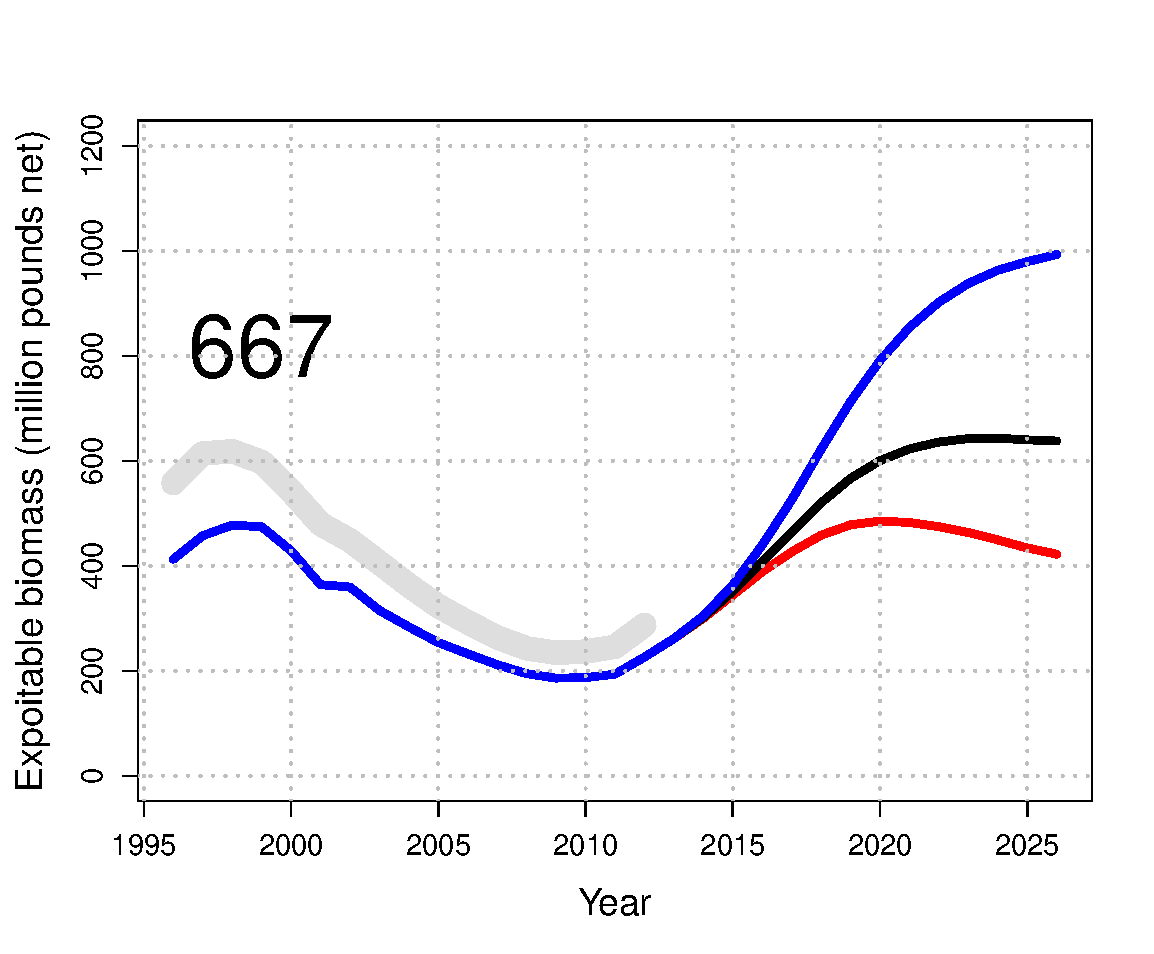
\includegraphics[height=1.5in]{../FIGURES/fig_SQUO_DI_EBio.pdf}
		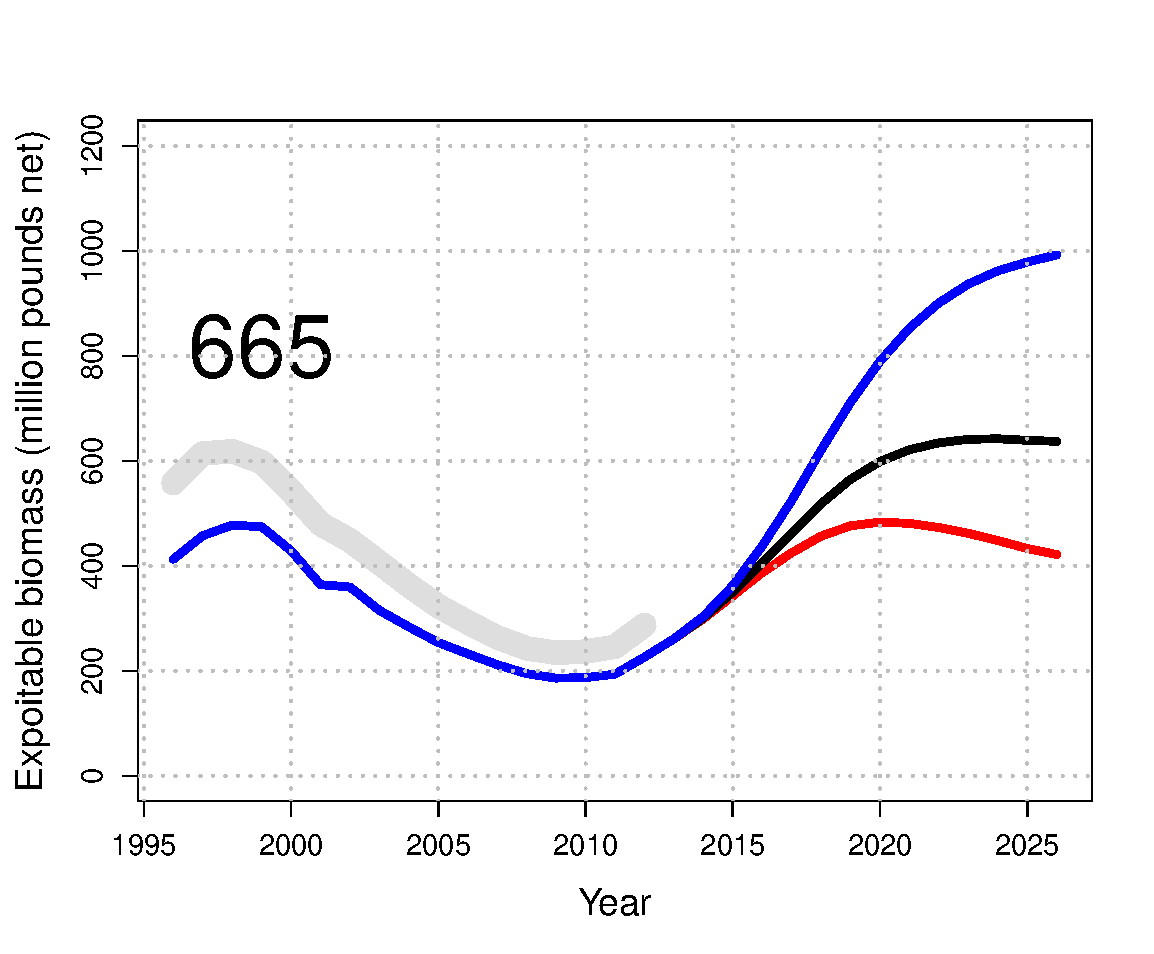
\includegraphics[height=1.5in]{../FIGURES/fig_BSAI_DI_EBio.pdf}
		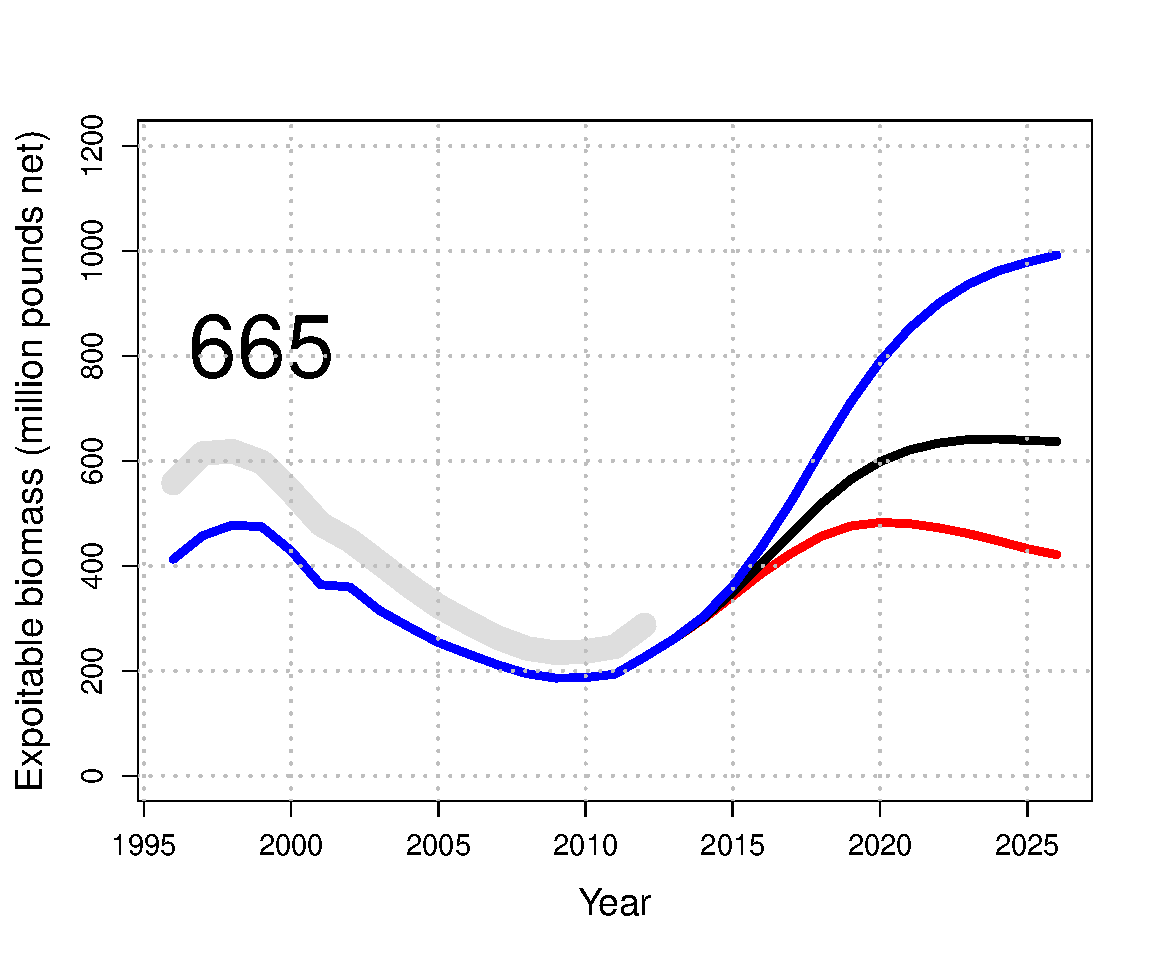
\includegraphics[height=1.5in]{../FIGURES/fig_GULF_DI_EBio.pdf}
		
		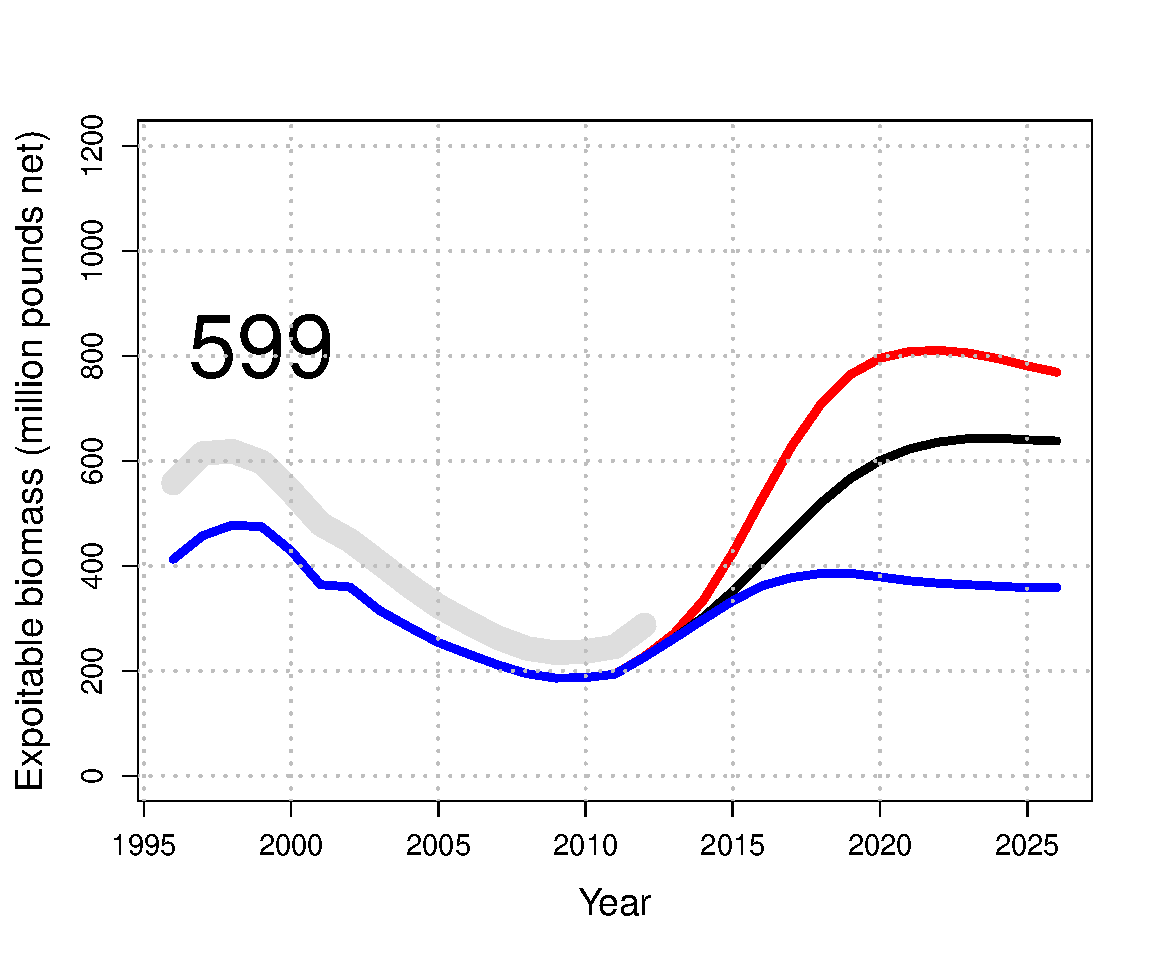
\includegraphics[height=1.5in]{../FIGURES/fig_SQUO_DD_EBio.pdf}
		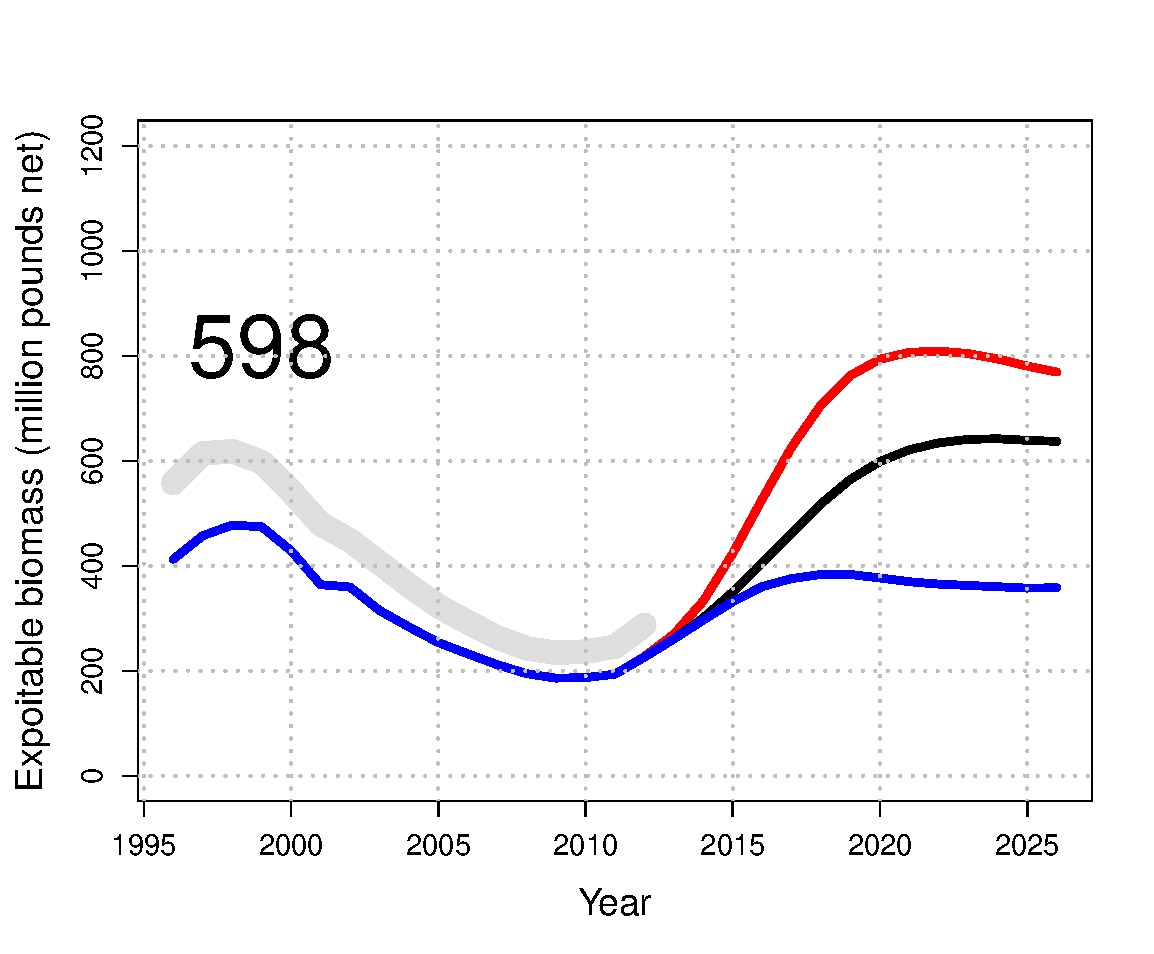
\includegraphics[height=1.5in]{../FIGURES/fig_BSAI_DD_EBio.pdf}
		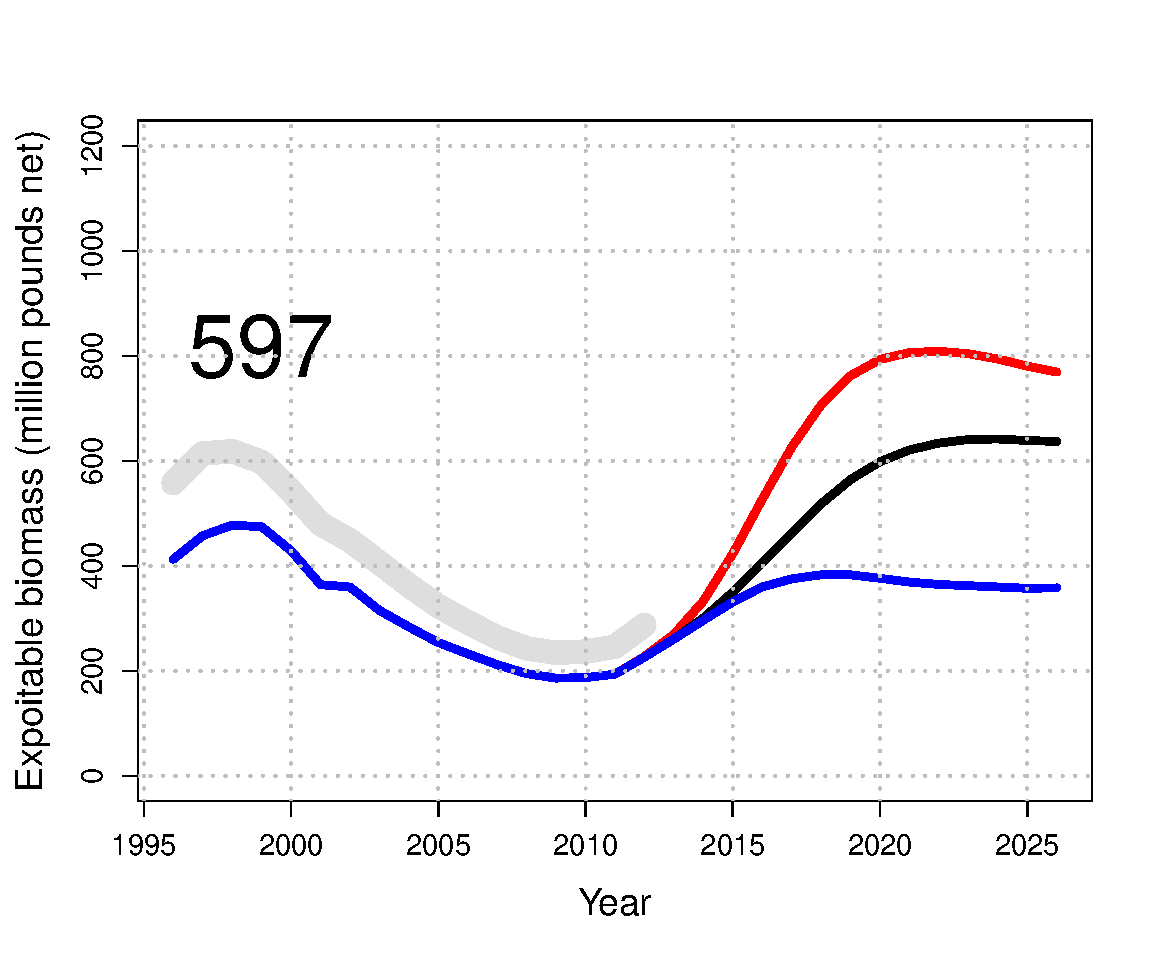
\includegraphics[height=1.5in]{../FIGURES/fig_GULF_DD_EBio.pdf}		
	\caption{Simulated coastwide exploitable  biomass under the assumptions of density-independent growth (top row) and density dependent growth (bottom row) for the Status Quo scenarios (left), 50\% bycatch reduction in BSAI (middle), and 50\% bycatch reduction in the GULF (right).  Poor, average, and good recruitment scenarios denoted with, red, black and blue lines, respectively.}
	\label{fig:FIGURES_fig_SQUO_DI_EBio}
\end{figure}

% subsection effects_of_bycatch_reduction_on_ebio (end)

% ----------------------------------------------------------------------------- %
\subsection{Effects of bycath reduction on Spawning biomass} % (fold)
\label{sub:effects_of_bycath_reduction_on_spawning_biomass}
Reducing bycatch in the BSAI and GULF fisheries also has little impact on the projected coastwide female spawning stock biomass (Figure \ref{fig:FIGURES_fig_SQUO_DI_SBio}).  Projected female spawning biomass ranges between 472 million lb. to 506 million lb. under density-dependent and density-independent growth scenarios, respectively.  The impacts of density-dependent growth on female spawning stock biomass is much less than the impacts on the exploitable biomass.  This is largely due to the addition of faster growing males (at low density) in the calculation of exploitable biomass.
\begin{figure}[htbp]
	\centering
		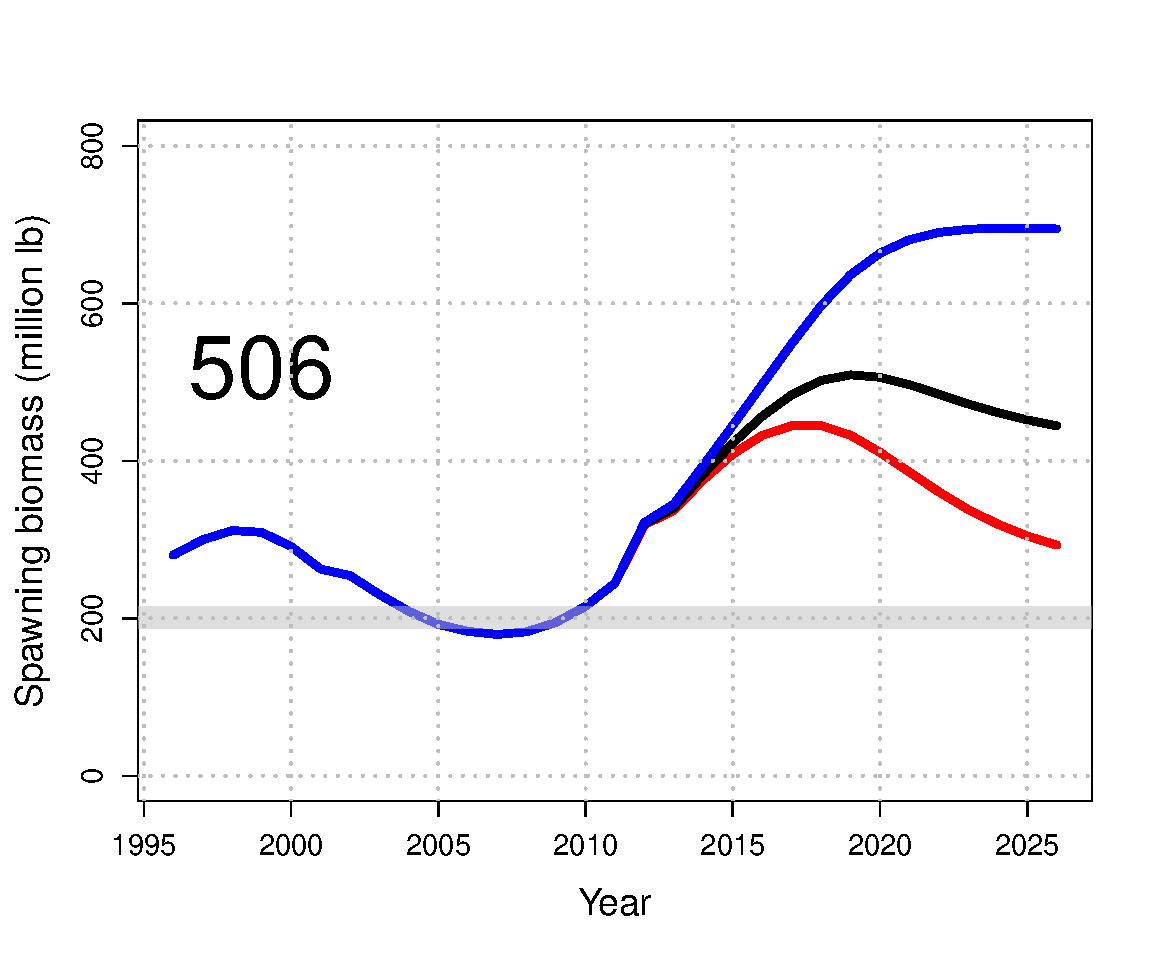
\includegraphics[height=1.5in]{../FIGURES/fig_SQUO_DI_SBio.pdf}
		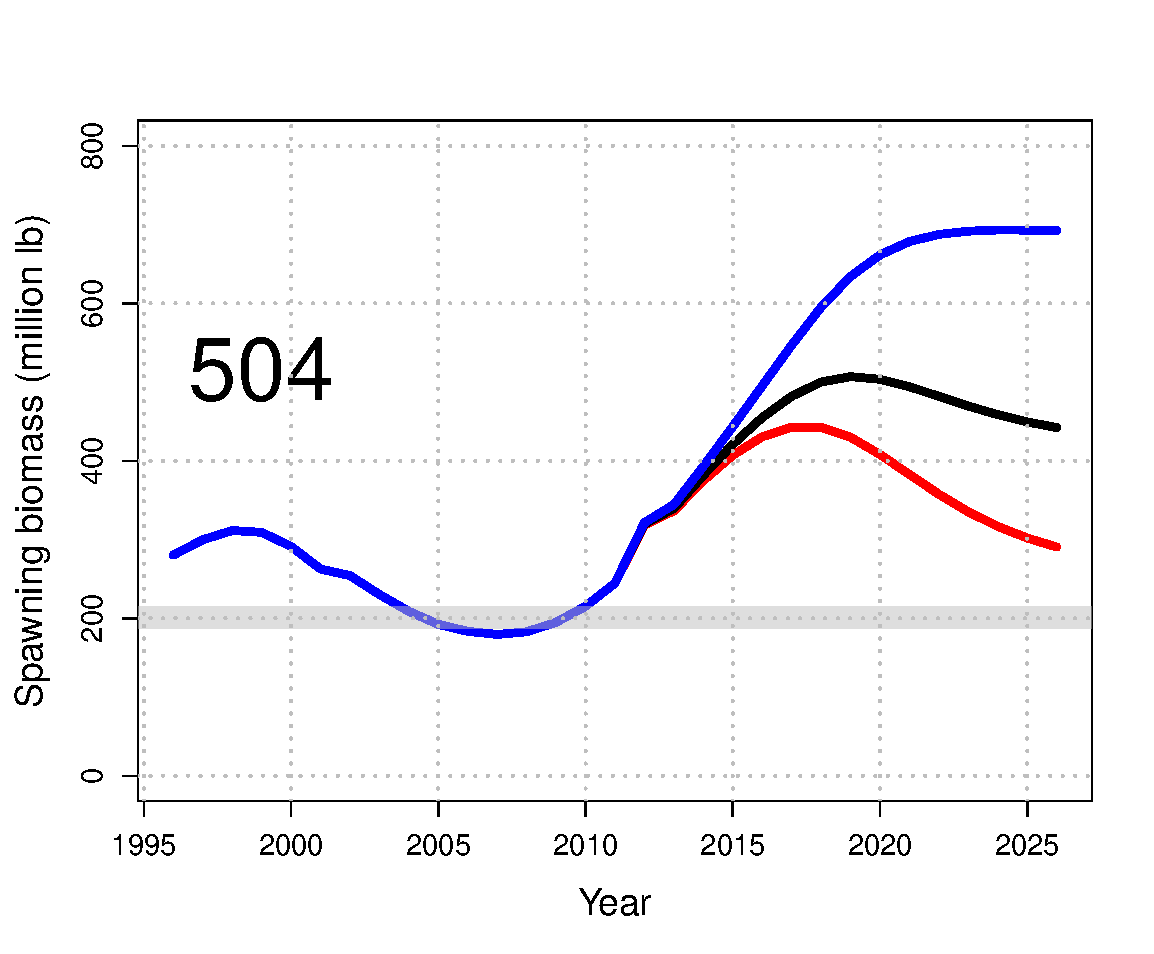
\includegraphics[height=1.5in]{../FIGURES/fig_BSAI_DI_SBio.pdf}
		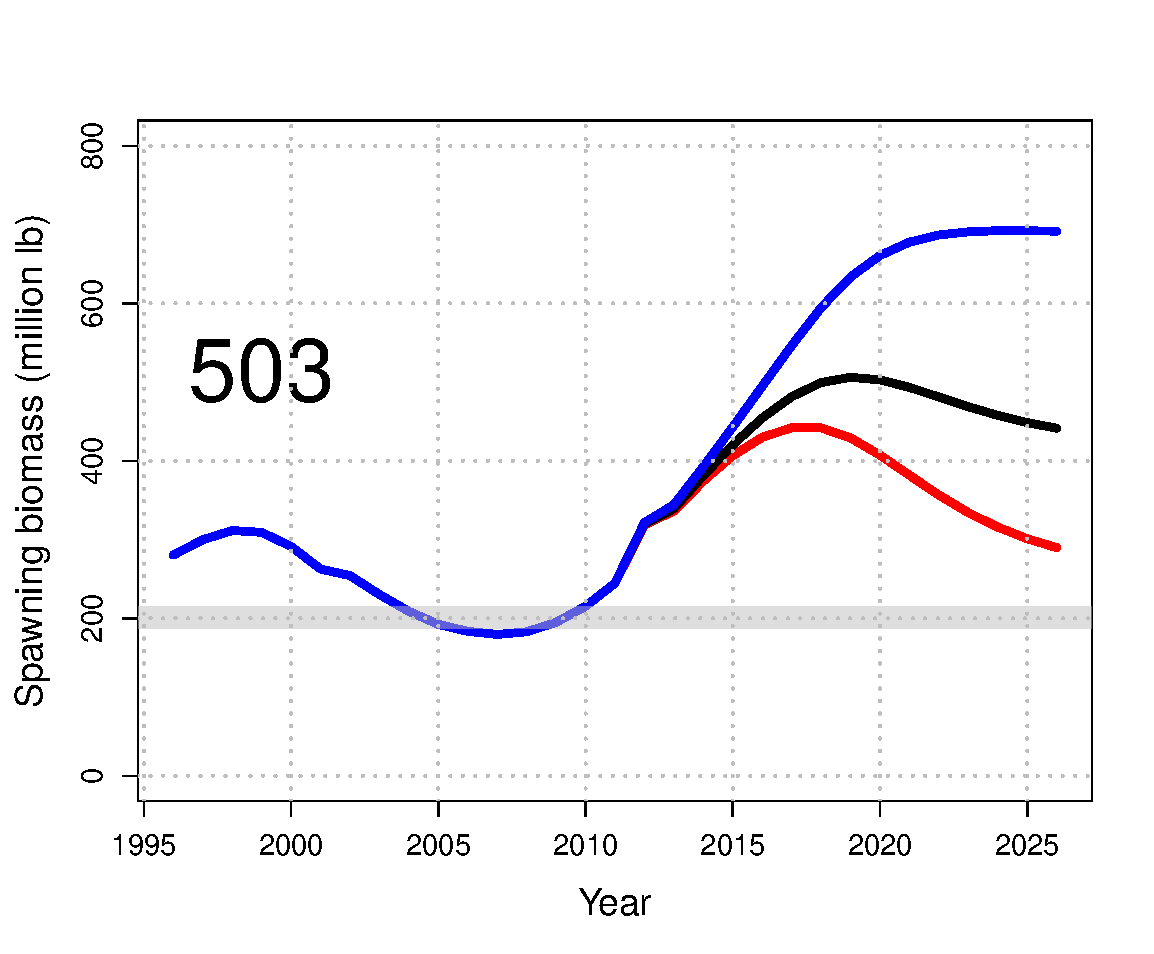
\includegraphics[height=1.5in]{../FIGURES/fig_GULF_DI_SBio.pdf}
		
		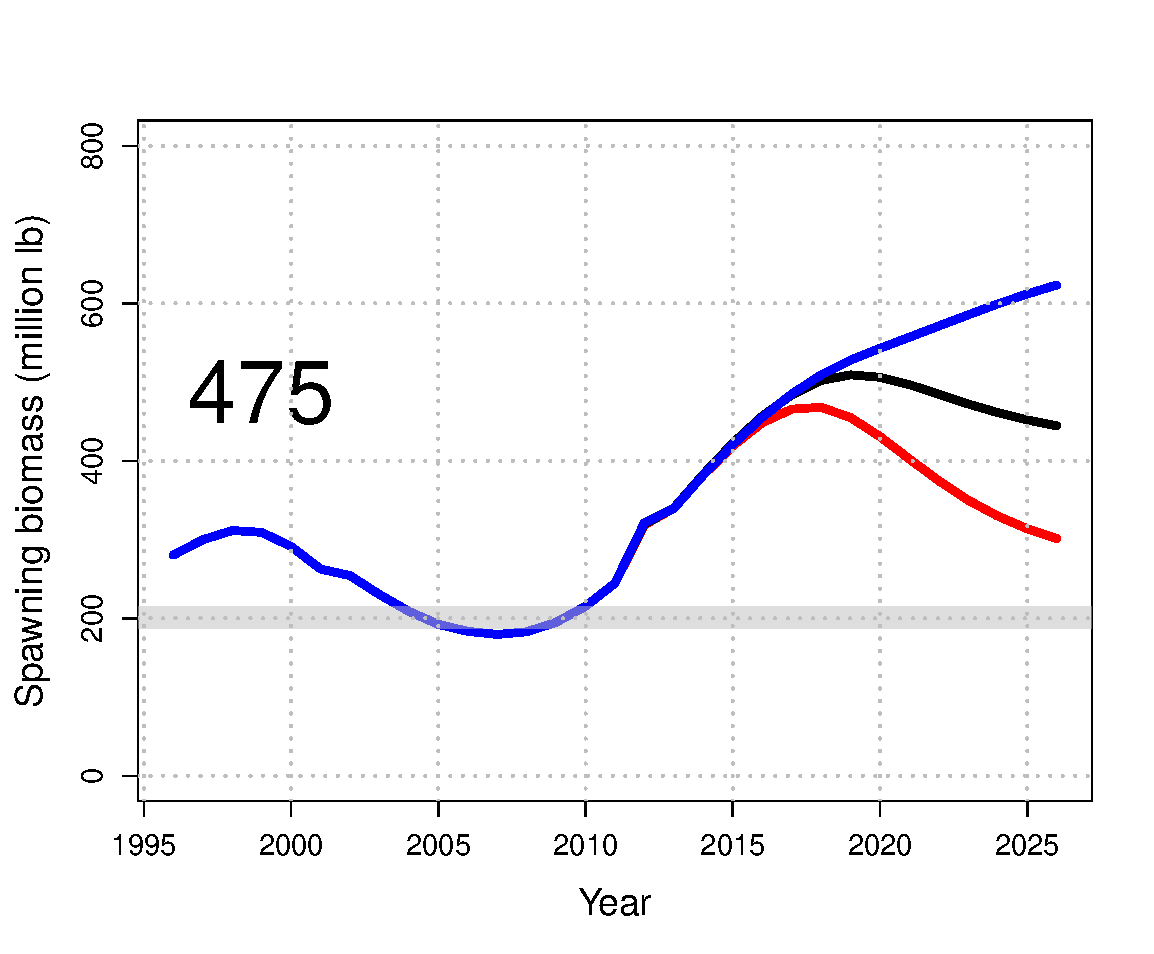
\includegraphics[height=1.5in]{../FIGURES/fig_SQUO_DD_SBio.pdf}
		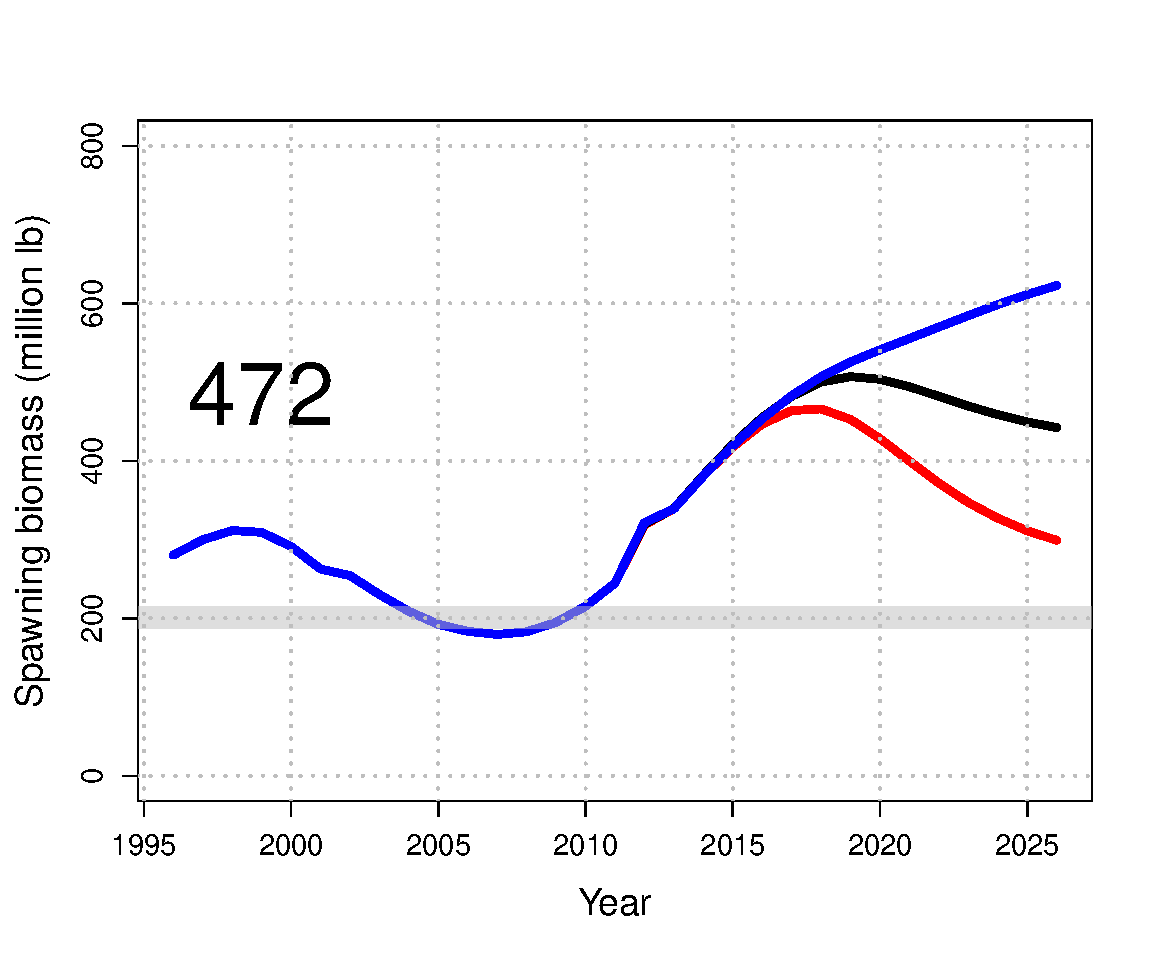
\includegraphics[height=1.5in]{../FIGURES/fig_BSAI_DD_SBio.pdf}
		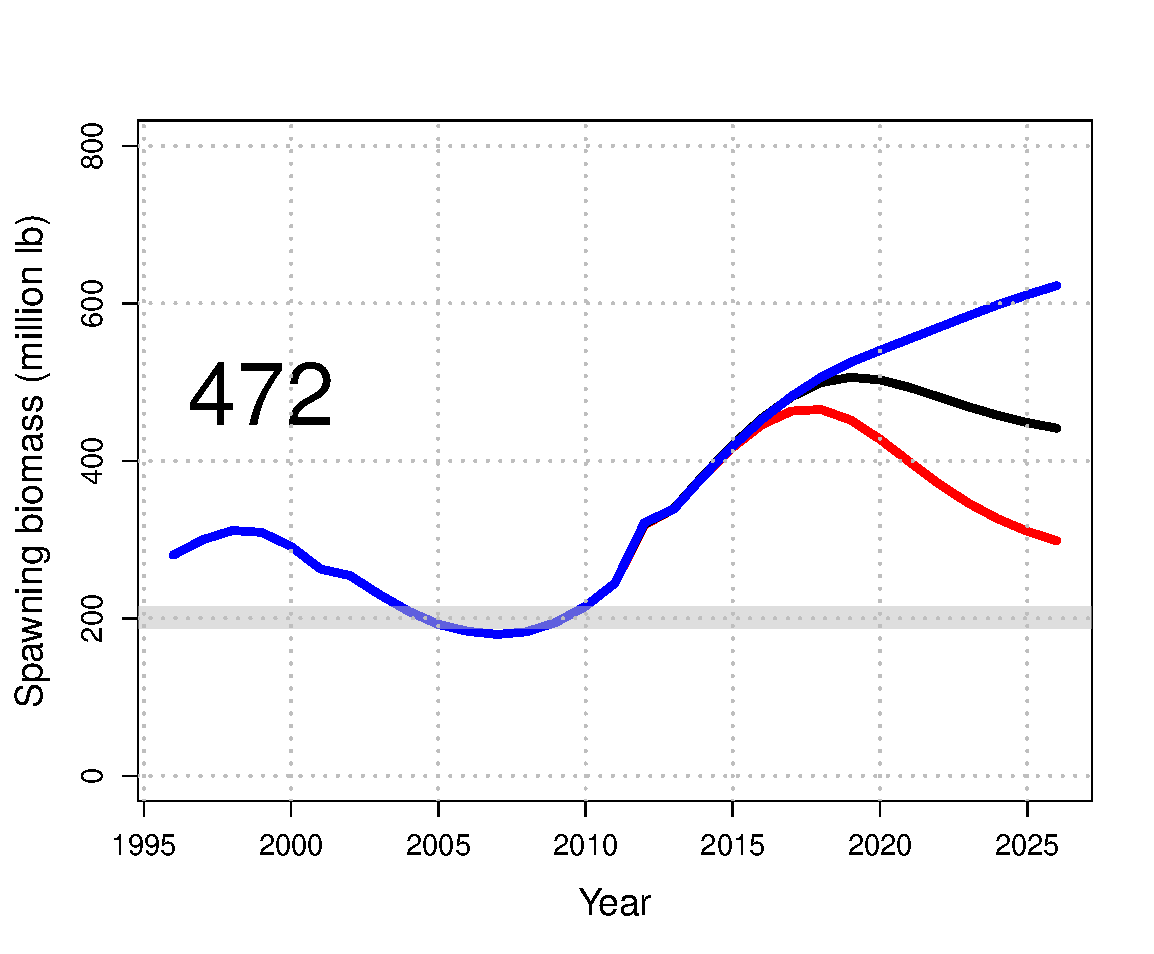
\includegraphics[height=1.5in]{../FIGURES/fig_GULF_DD_SBio.pdf}
	\caption{Simulated coastwide female spawning biomass under the assumptions of density-independent growth (top row) and density dependent growth (bottom row) for the Status Quo scenarios (left), 50\% bycatch reduction in BSAI (middle), and 50\% bycatch reduction in the GULF (right).  Poor, average, and good recruitment scenarios denoted with, red, black and blue lines, respectively.}
	\label{fig:FIGURES_fig_SQUO_DI_SBio}
\end{figure}

% subsection effects_of_bycath_reduction_on_spawning_biomass (end)

% ----------------------------------------------------------------------------- %
\subsection{Effects of bycatch reduction on commercial yield} % (fold)
\label{sub:effects_of_bycatch_reduction_on_commercial_yield}
The effects of reducing commercial bycatch in BSAI or the GULF by roughly 2.7 million lbs. on the commercial yield is roughly a 2 million lb. increase in the commercial catch (Figure \ref{fig:FIGURES_fig_SQUO_DI_YBio}).  There is not a corresponding 1:1 increase in coastwide commercial yields with a reduction in bycatch in BSAI or the GULF management areas because the yield loss ratio (loss in commercial yield:bycatch) is less than 1 (Figure \ref{fig:FIGURES_YLR_fig_SQUO_DI_ylr}).


\begin{figure}[htbp]
	\centering
		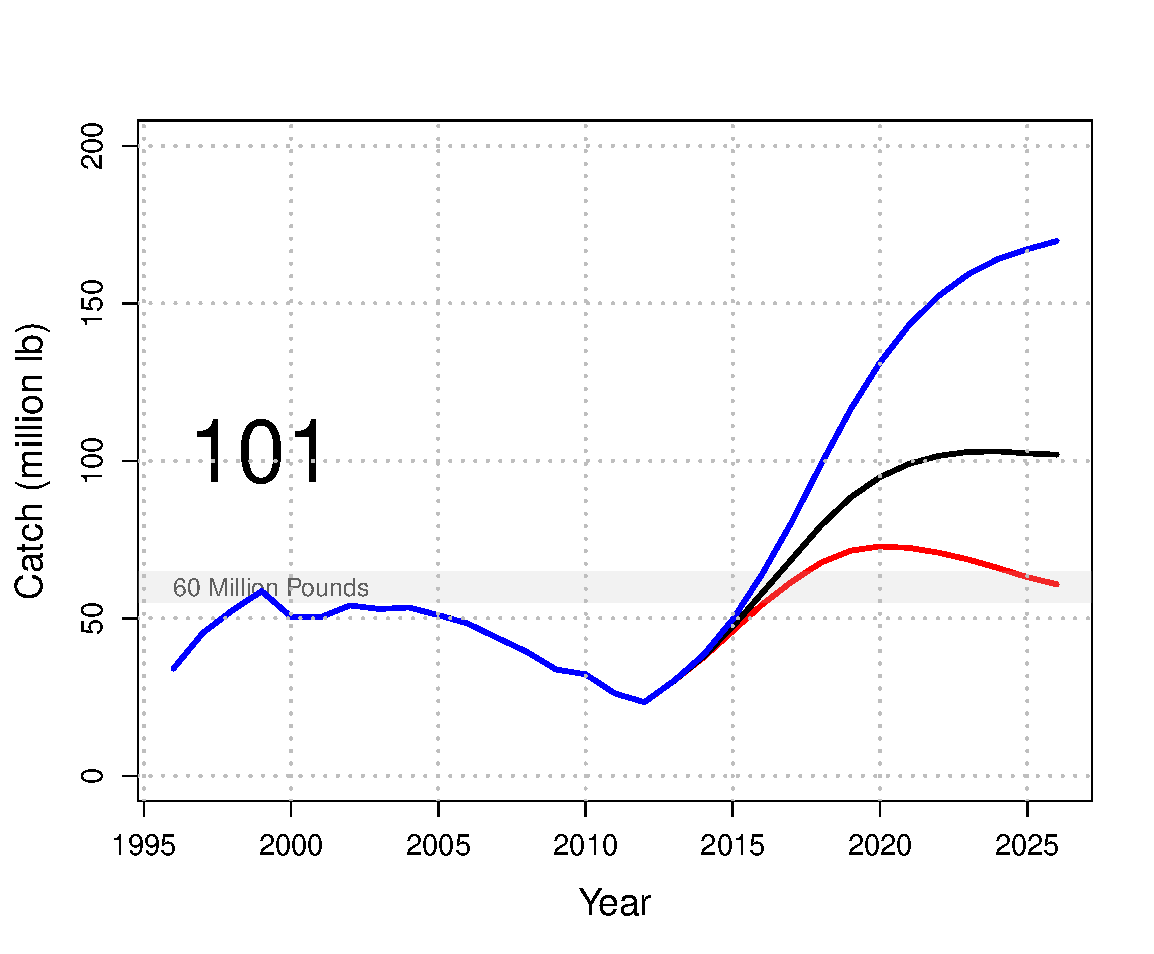
\includegraphics[height=1.5in]{../FIGURES/fig_SQUO_DI_YBio.pdf}
		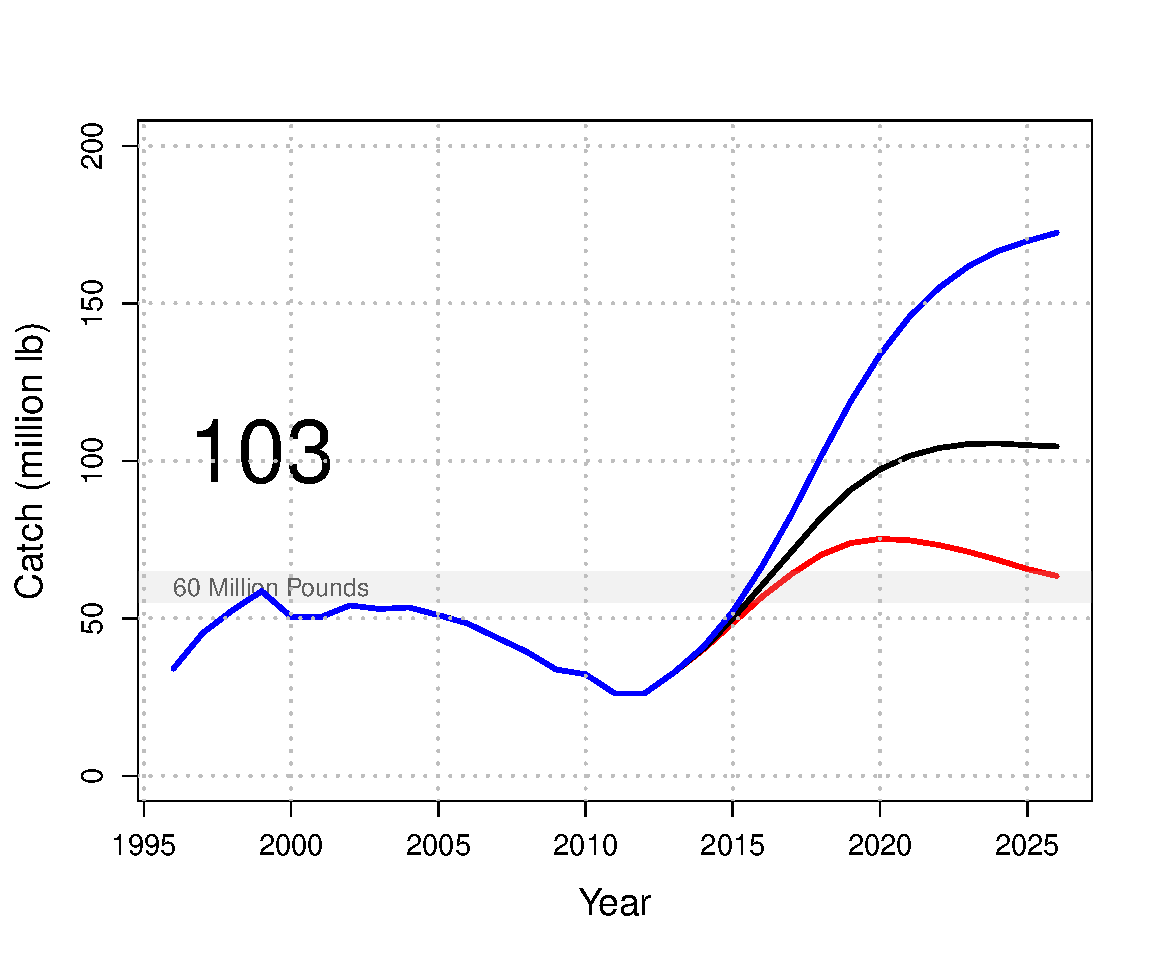
\includegraphics[height=1.5in]{../FIGURES/fig_BSAI_DI_YBio.pdf}
		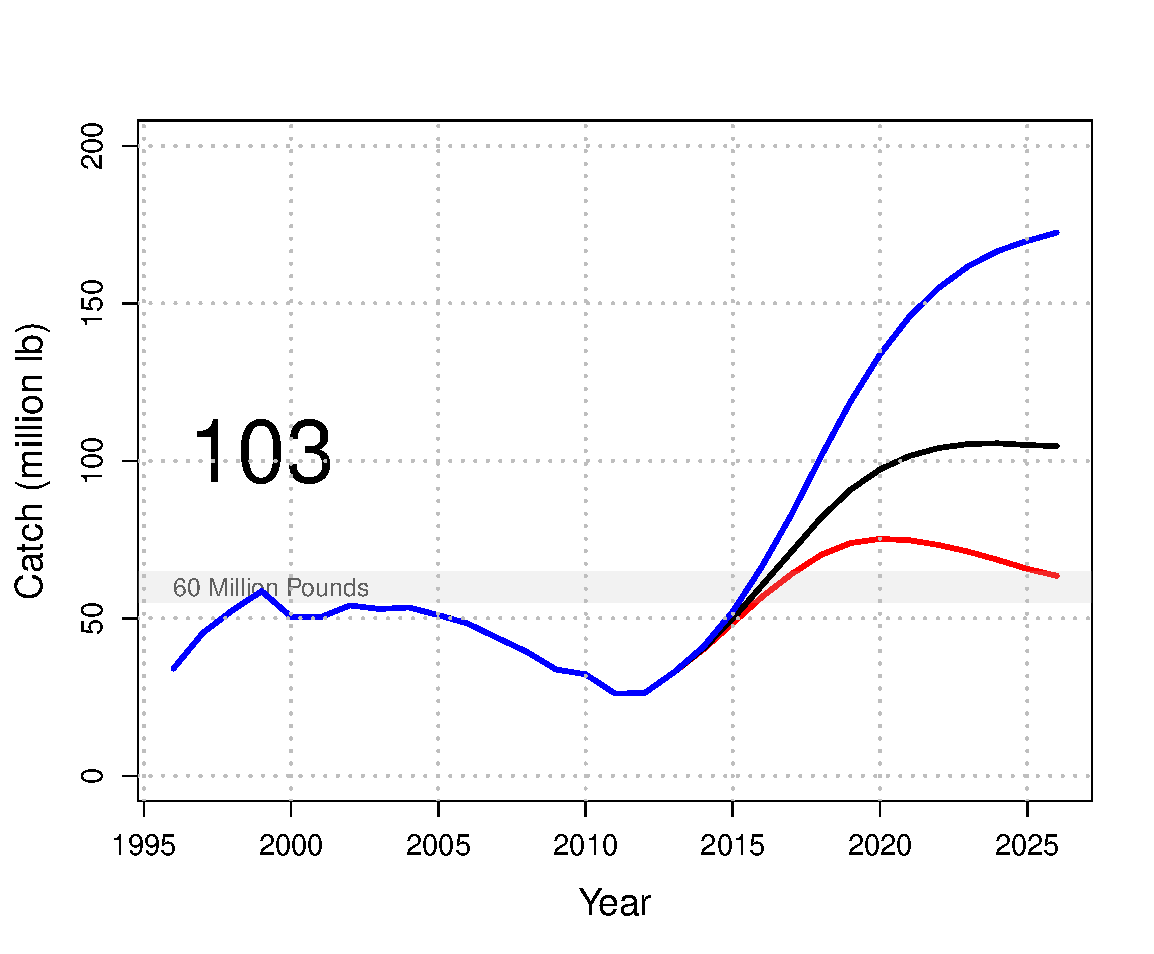
\includegraphics[height=1.5in]{../FIGURES/fig_GULF_DI_YBio.pdf}
		
		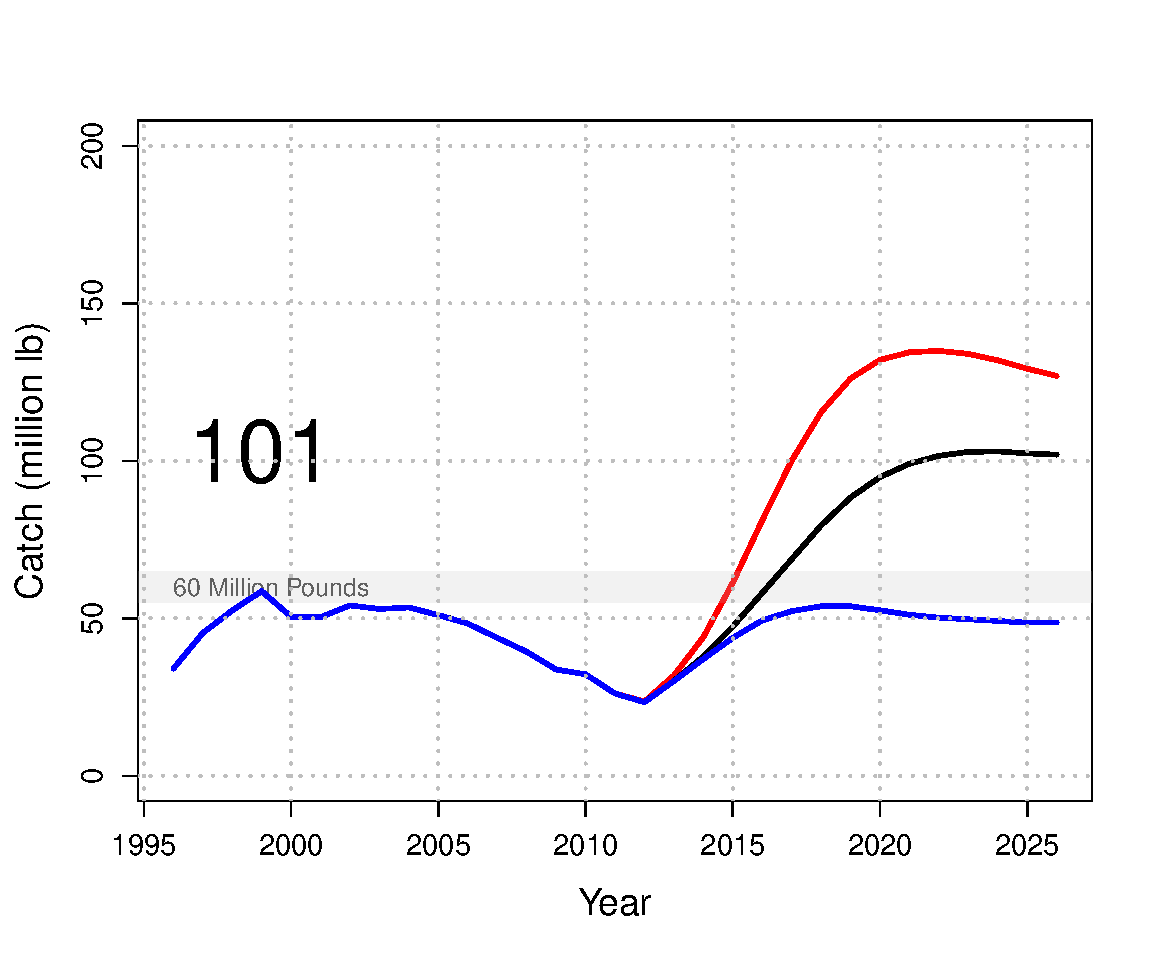
\includegraphics[height=1.5in]{../FIGURES/fig_SQUO_DD_YBio.pdf}
		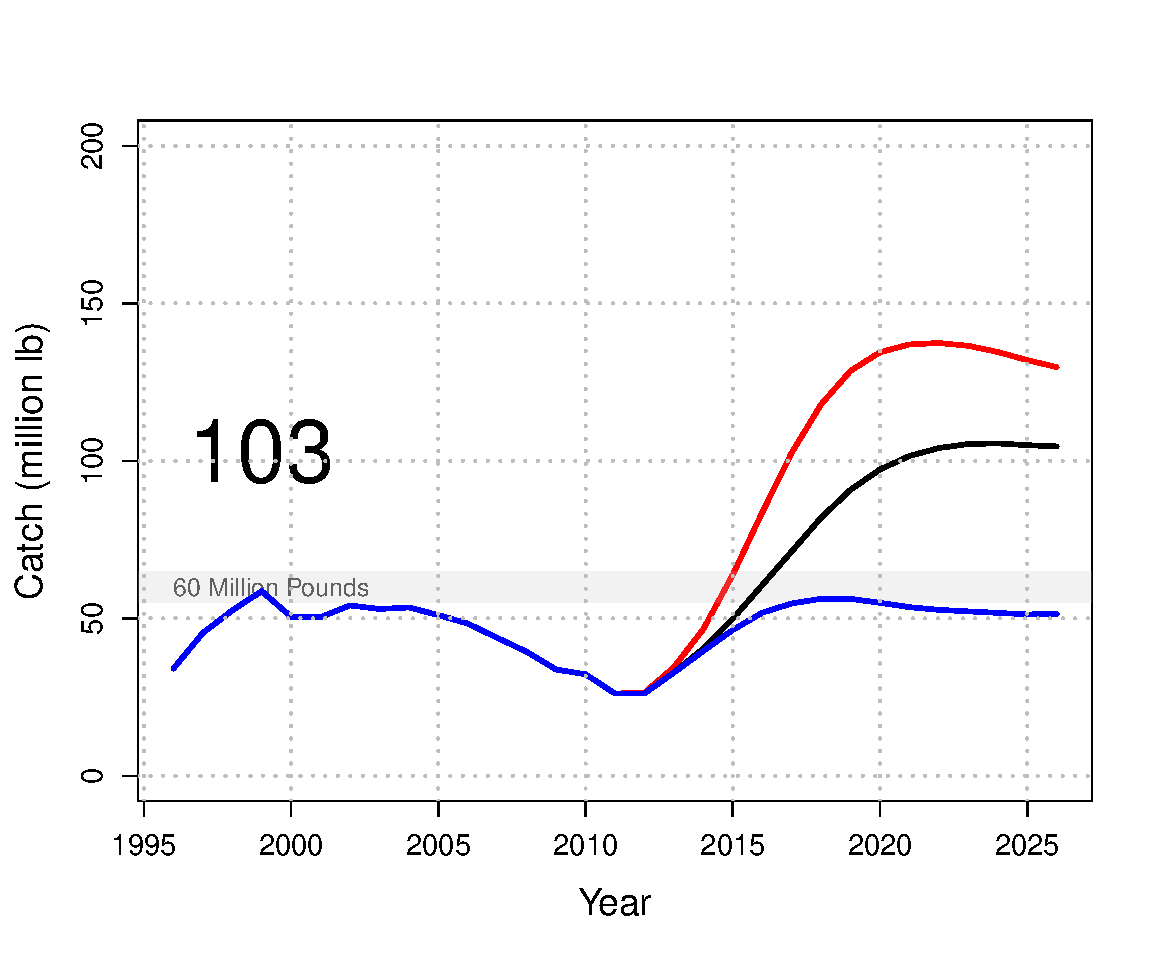
\includegraphics[height=1.5in]{../FIGURES/fig_BSAI_DD_YBio.pdf}
		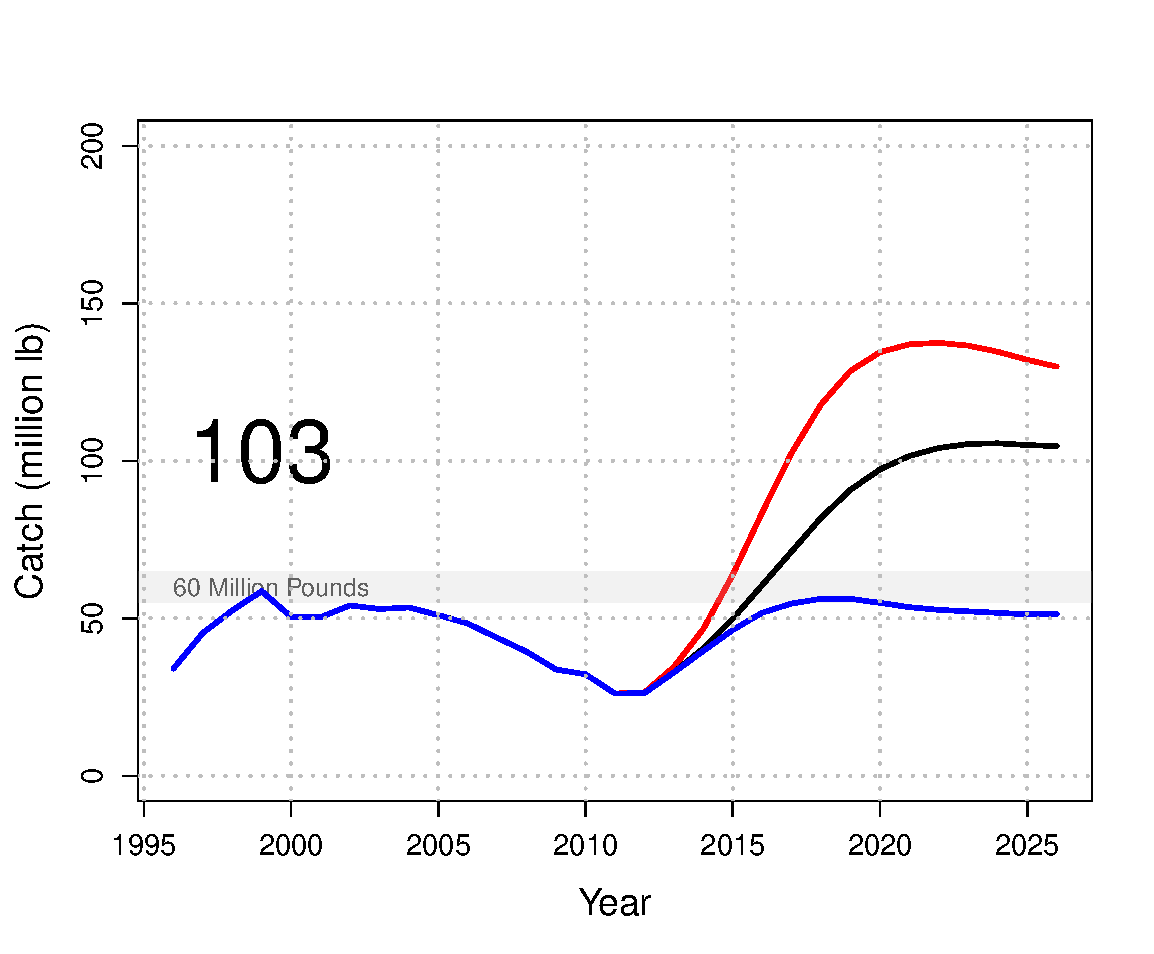
\includegraphics[height=1.5in]{../FIGURES/fig_GULF_DD_YBio.pdf}
	\caption{Simulated coastwide commercial yield under the assumptions of density-independent growth (top row) and density dependent growth (bottom row) for the Status Quo scenarios (left), 50\% bycatch reduction in BSAI (middle), and 50\% bycatch reduction in the GULF (right).  Poor, average, and good recruitment scenarios denoted with, red, black and blue lines, respectively.}
	\label{fig:FIGURES_fig_SQUO_DI_YBio}
\end{figure}

Trends in the yield loss ratios under constant growth assumptions are very similar due to stabilizing biomass-at-age in the simulated populations.  However, under the density-dependent growth hypotheses trends in the yield loss ratios differ markedly.  With reduced growth rates, the yield loss ratios are less than scenarios with increased growth rates.  In short, there is some compensation in the yield  associated with increased growth rates at low density.  There is however, no substantial difference in the yield loss ratios with decreasing the bycatch rates in BSAI or the GULF regions (Figure \ref{fig:FIGURES_YLR_fig_SQUO_DI_ylr}).

\begin{figure}[htbp]
	\centering
		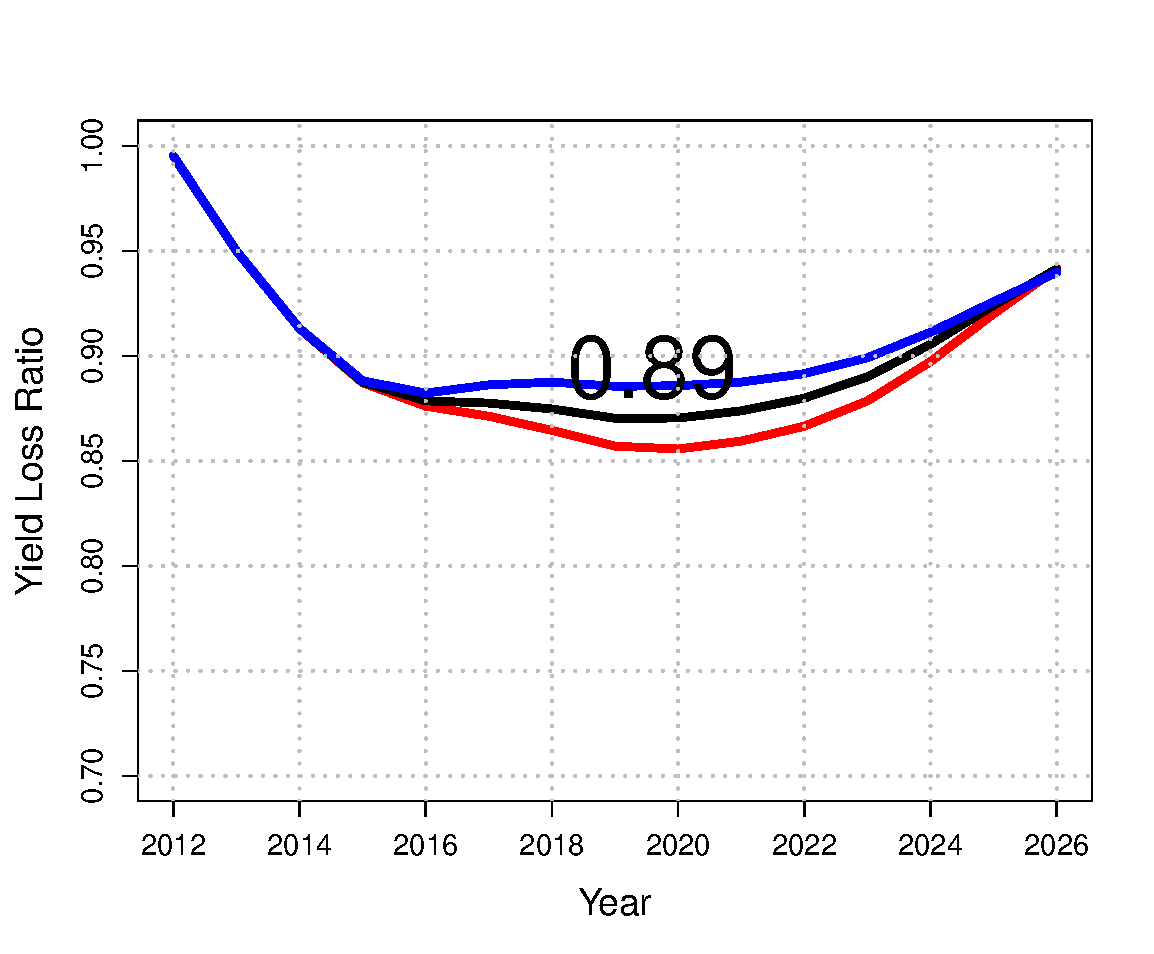
\includegraphics[height=1.5in]{../FIGURES/YLR/fig_SQUO_DI_ylr.pdf}
		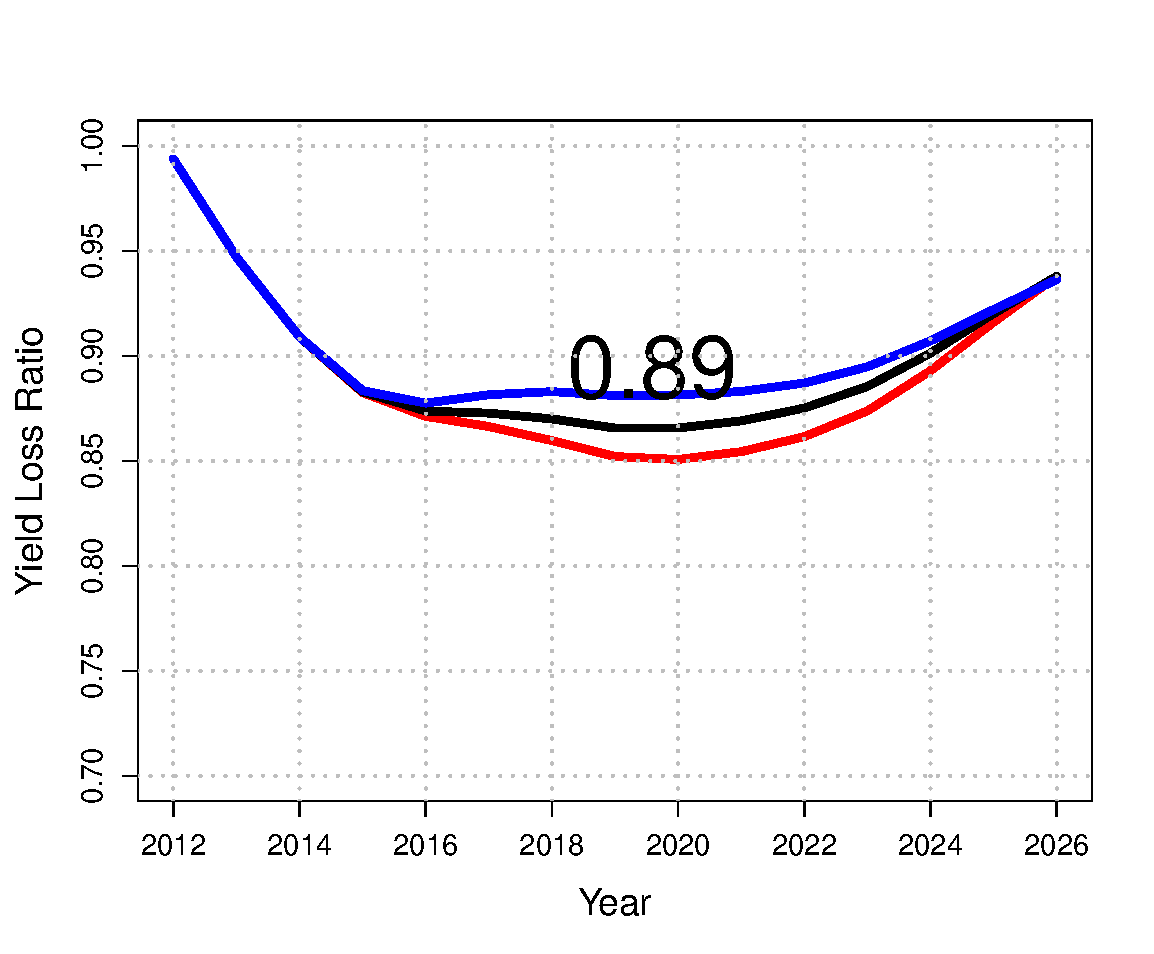
\includegraphics[height=1.5in]{../FIGURES/YLR/fig_BSAI_DI_ylr.pdf}
		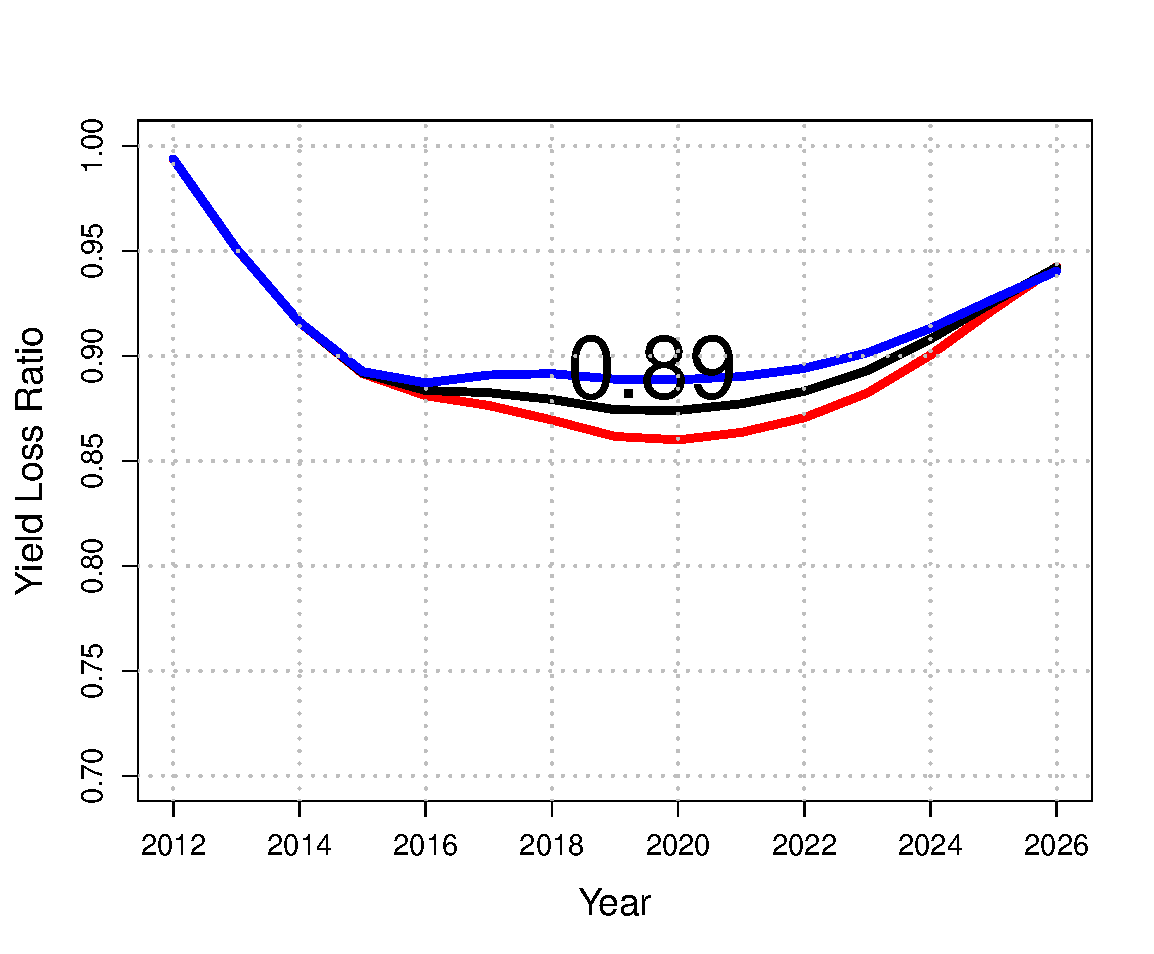
\includegraphics[height=1.5in]{../FIGURES/YLR/fig_GULF_DI_ylr.pdf}
                                
		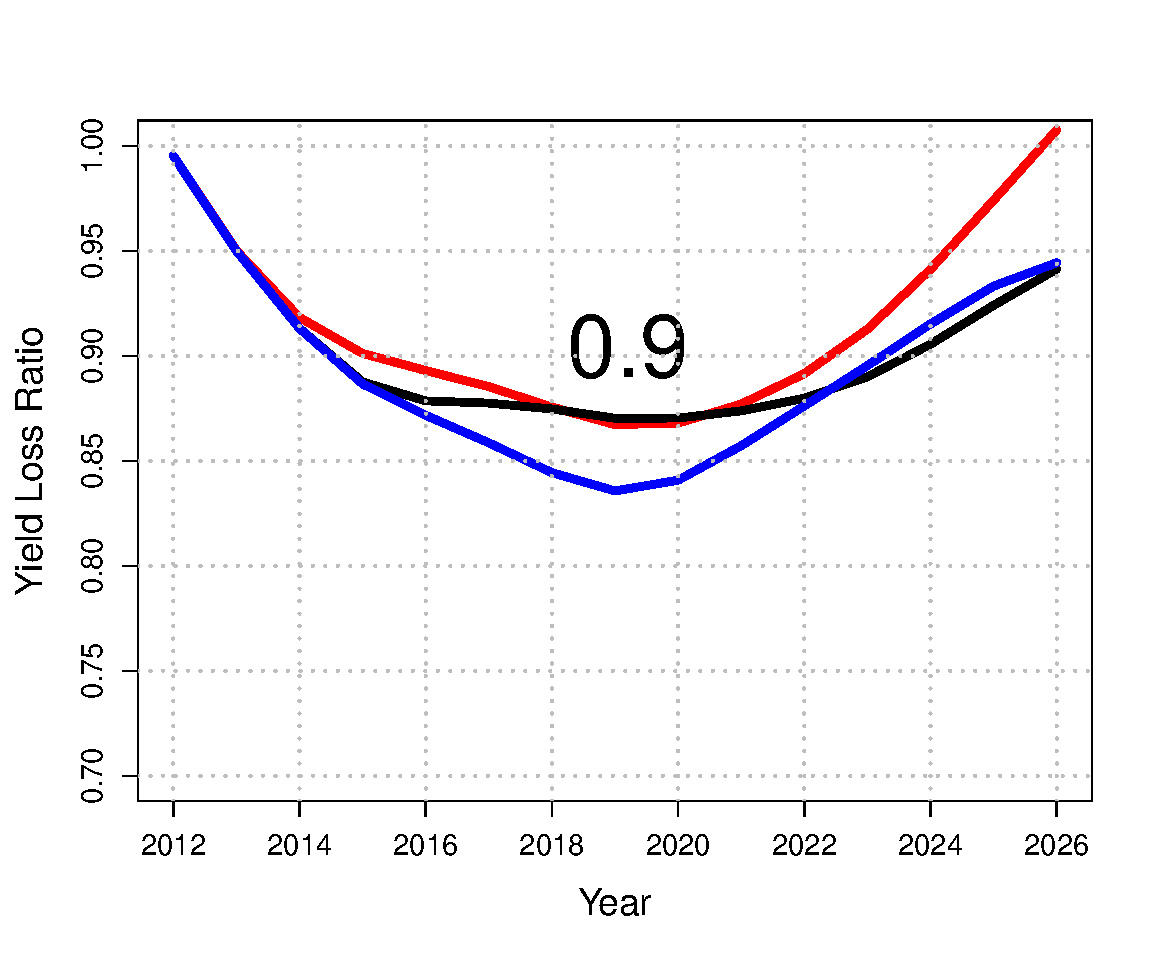
\includegraphics[height=1.5in]{../FIGURES/YLR/fig_SQUO_DD_ylr.pdf}
		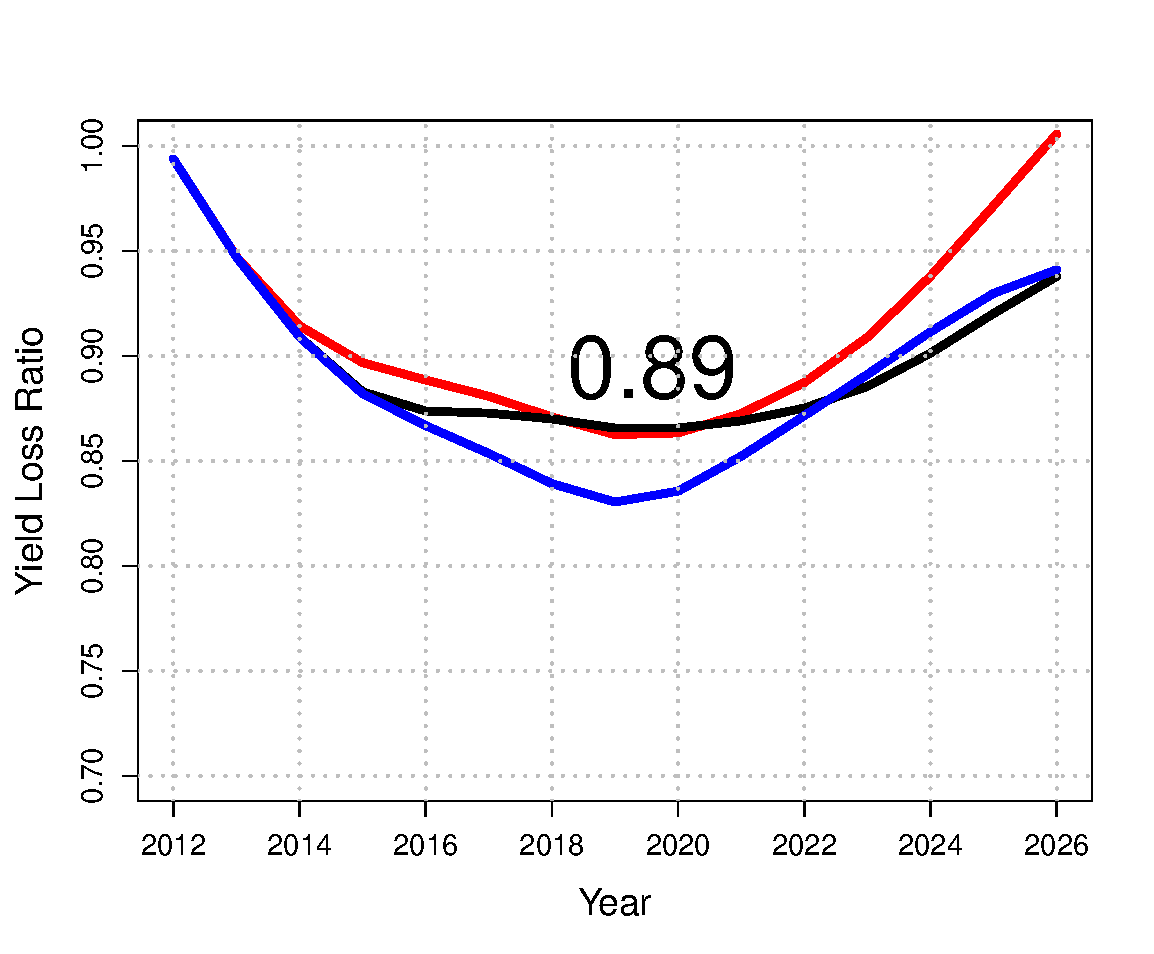
\includegraphics[height=1.5in]{../FIGURES/YLR/fig_BSAI_DD_ylr.pdf}
		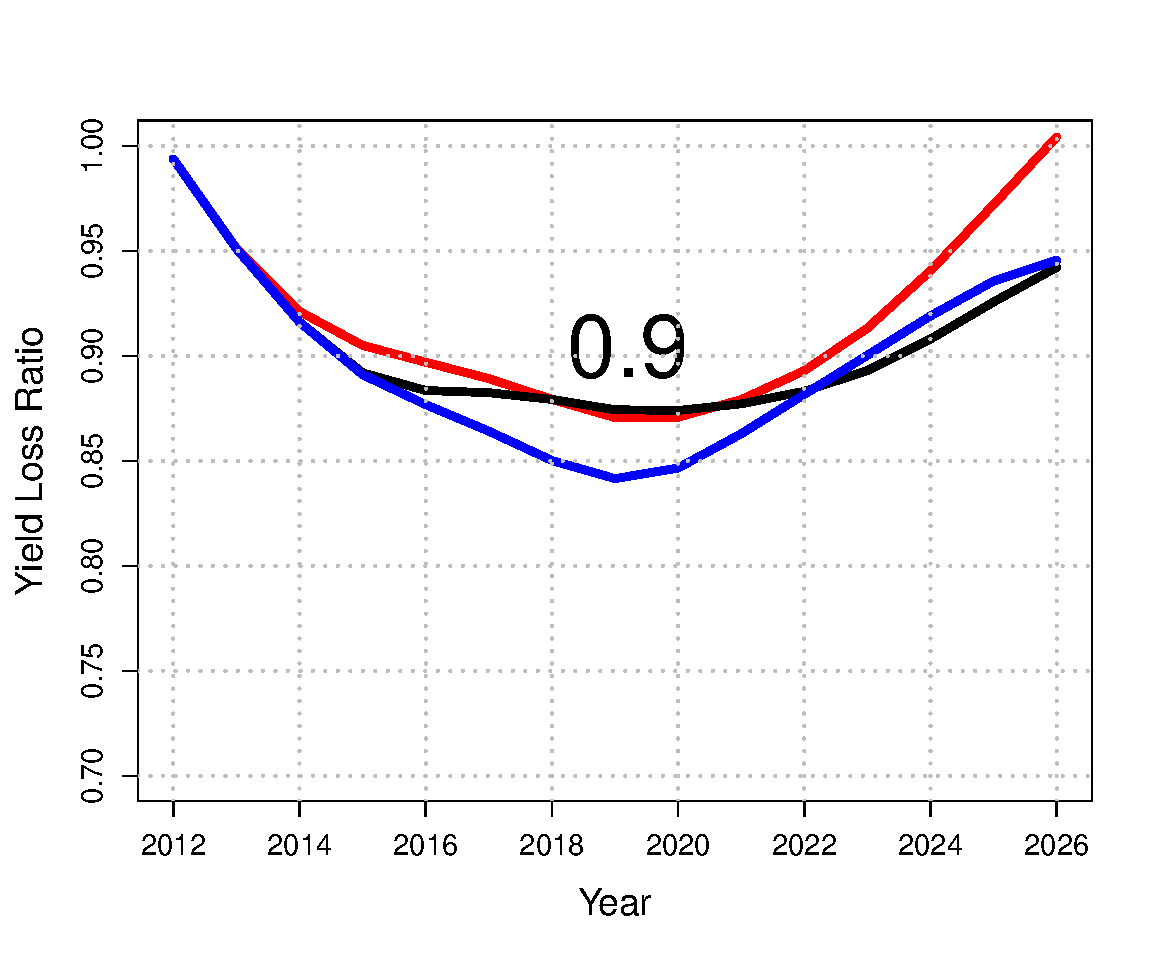
\includegraphics[height=1.5in]{../FIGURES/YLR/fig_GULF_DD_ylr.pdf}		
	\caption{Simulated coastwide commercial yield loss ratios under the assumptions of density-independent growth (top row) and density dependent growth (bottom row) for the Status Quo scenarios (left), 50\% bycatch reduction in BSAI (middle), and 50\% bycatch reduction in the GULF (right).  Poor, average, and good recruitment scenarios denoted with, red, black and blue lines, respectively.}
	\label{fig:FIGURES_YLR_fig_SQUO_DI_ylr}
\end{figure}
% subsection effects_of_bycatch_reduction_on_commercial_yield (end)

% ----------------------------------------------------------------------------- %
\subsection{Effects of bycatch reduction on commercial wastage} % (fold)
\label{sub:effects_of_bycatch_reduction_on_commercial_wastage}

The modest increases in commercial yield associated with bycatch reduction in the non-targeted fisheries results in a corresponding increase in commercial waste.  Waste increases from an average of 2.796 million pounds to 2.891 million pounds under the density independent growth hypotheses (Figure \ref{fig:FIGURES_fig_SQUO_DI_WBio}).  Under the density dependent growth hypothesis wastage increases from 2.192 million pounds to 2.287 million pounds.  At low recruitment densities, increasing growth rates actually result in reduced wastage under the current size limit of 26 inches (81.28 cm).

\begin{figure}[htbp]
	\centering
		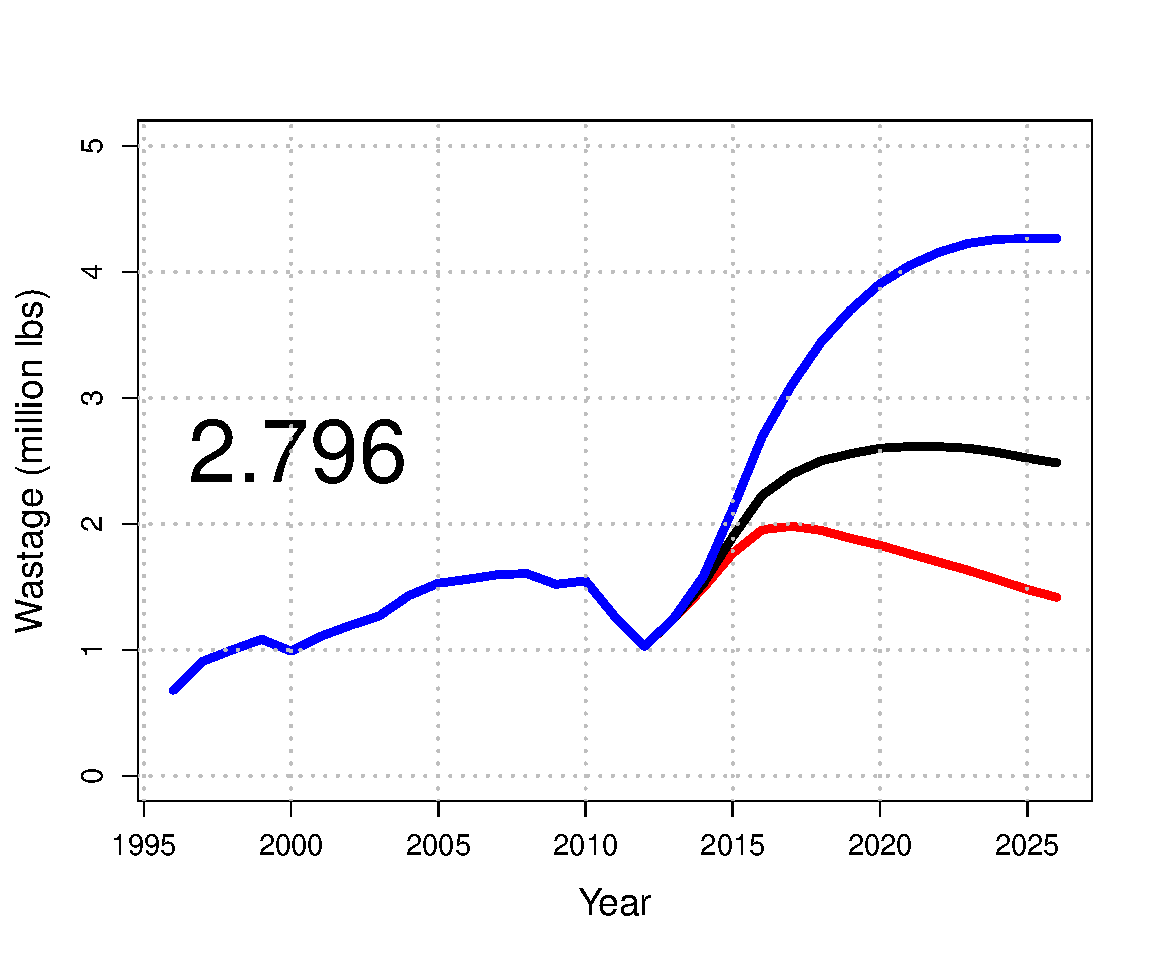
\includegraphics[height=1.5in]{../FIGURES/fig_SQUO_DI_WBio.pdf}
		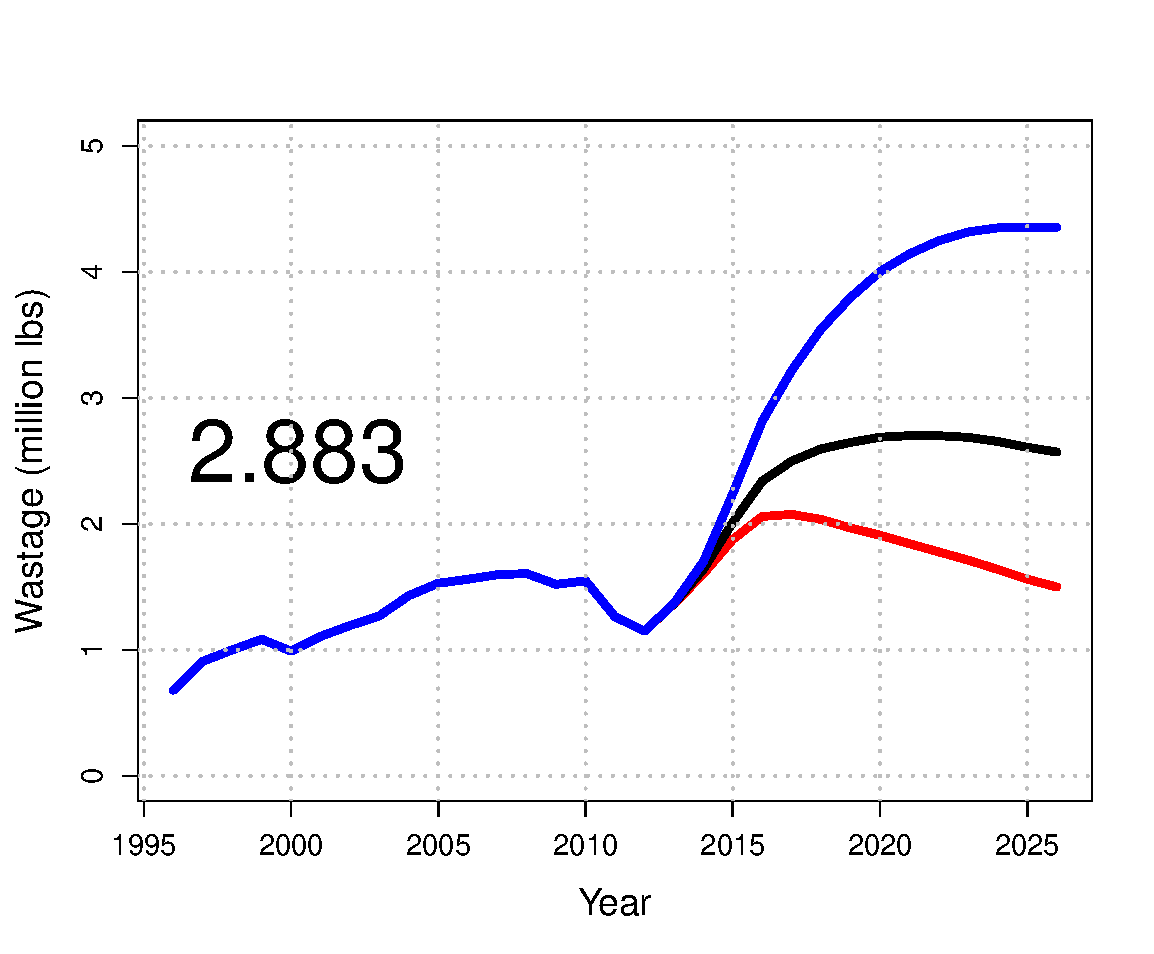
\includegraphics[height=1.5in]{../FIGURES/fig_BSAI_DI_WBio.pdf}
		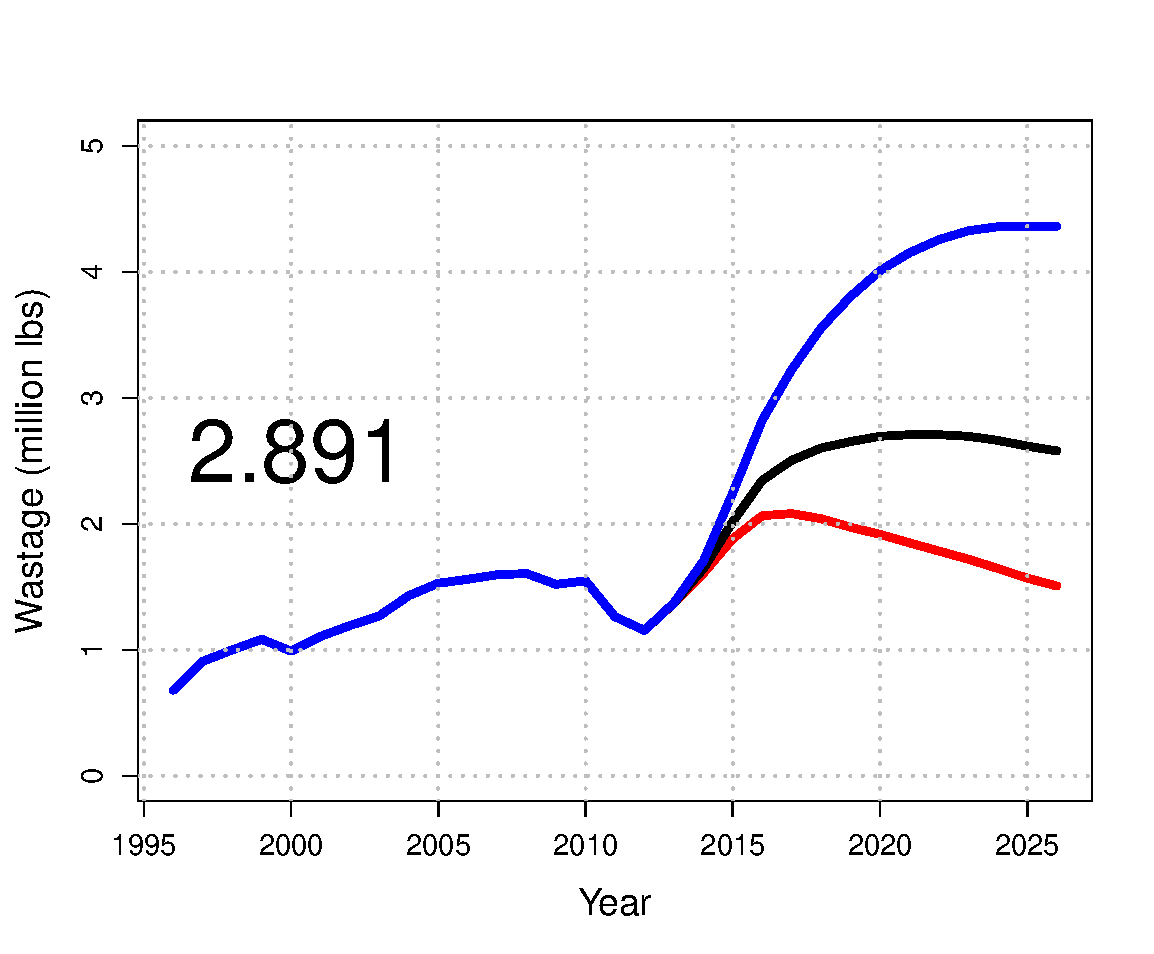
\includegraphics[height=1.5in]{../FIGURES/fig_GULF_DI_WBio.pdf}
		
		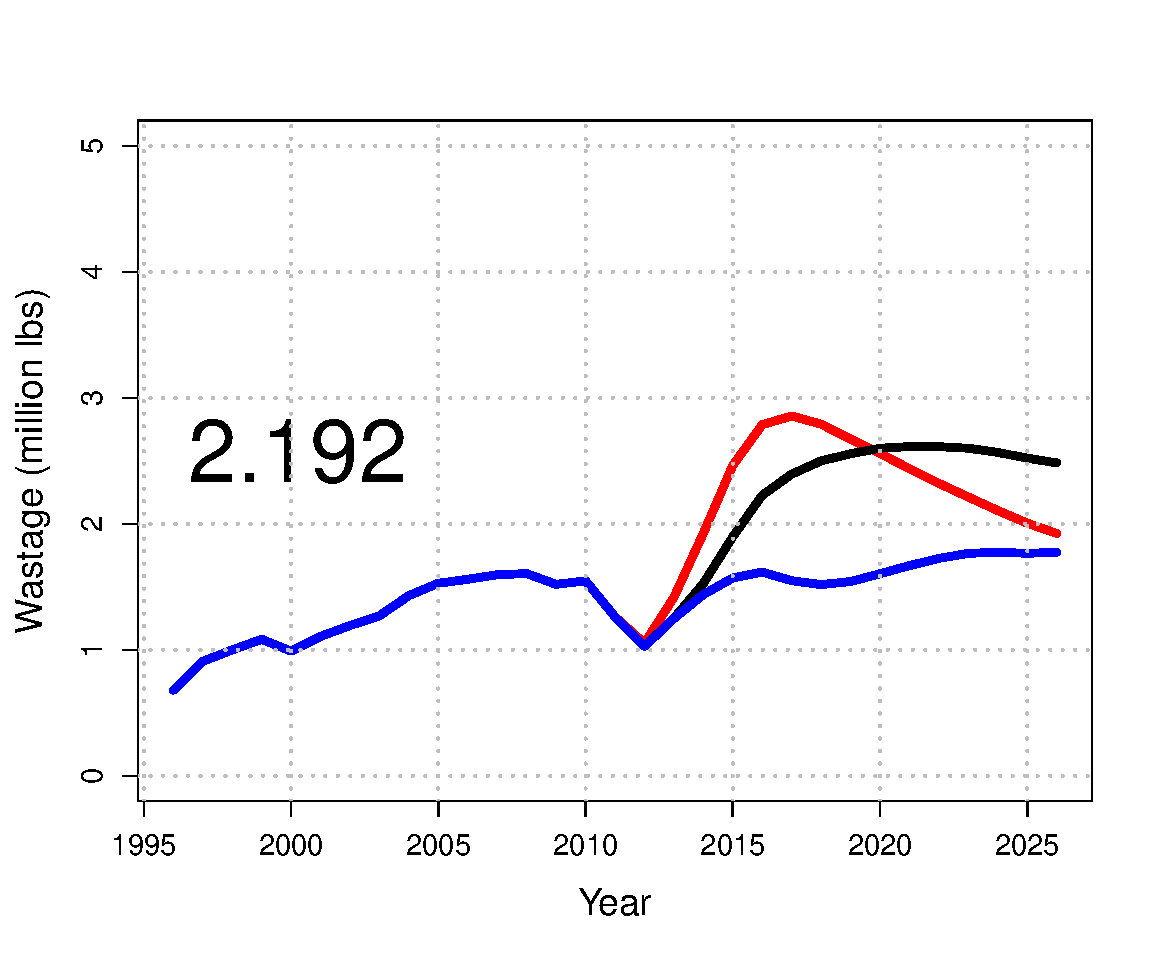
\includegraphics[height=1.5in]{../FIGURES/fig_SQUO_DD_WBio.pdf}
		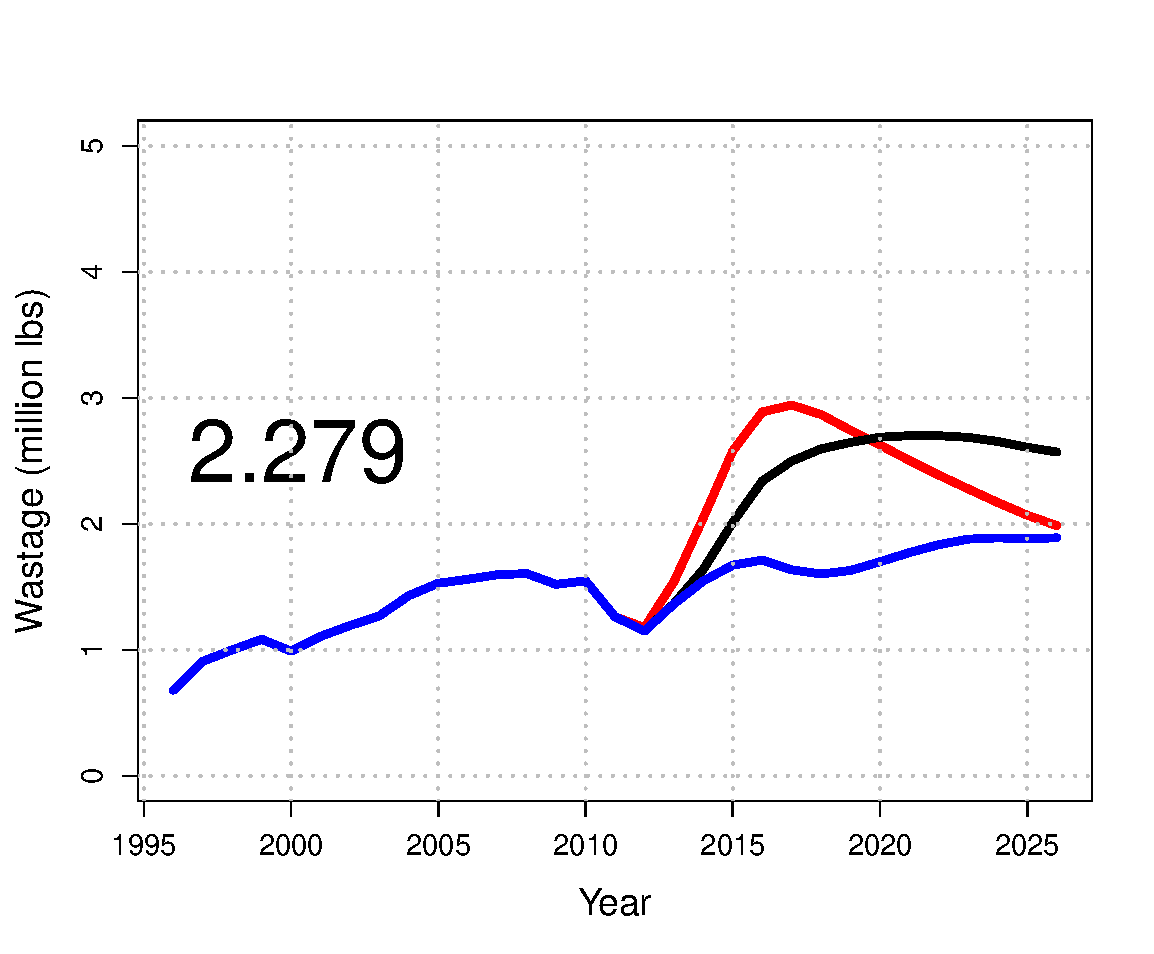
\includegraphics[height=1.5in]{../FIGURES/fig_BSAI_DD_WBio.pdf}
		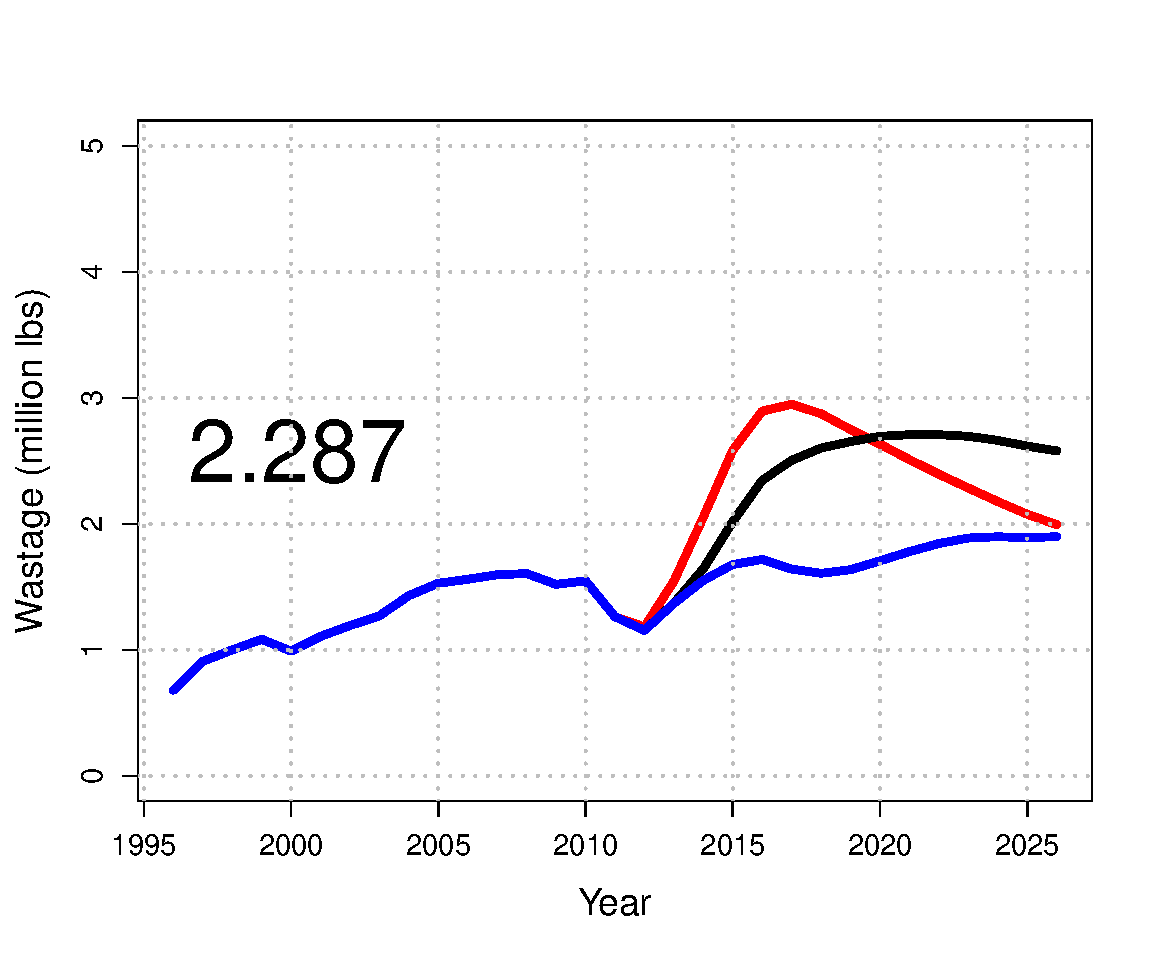
\includegraphics[height=1.5in]{../FIGURES/fig_GULF_DD_WBio.pdf}
	\caption{Simulated coastwide wastage from the commercial fishery under the assumptions of density-independent growth (top row) and density dependent growth (bottom row) for the Status Quo scenarios (left), 50\% bycatch reduction in BSAI (middle), and 50\% bycatch reduction in the GULF (right).  Poor, average, and good recruitment scenarios denoted with, red, black and blue lines, respectively.}
	\label{fig:FIGURES_fig_SQUO_DI_WBio}
\end{figure}


% subsection effects_of_bycatch_reduction_on_commercial_wastage (end)


% section results (end)




















